% Informe final (etapa 4) del Reto SIMA - Equipo 1, Grupo 201, MA2003B
% Compilar con pdfLaTeX (Overleaf: compilador pdfLaTeX). Fuente del contenido: quarto/etapa4_informe_final.qmd (main).
\documentclass[11pt,letterpaper]{article}

\usepackage[T1]{fontenc}
\usepackage[utf8]{inputenc}
\usepackage[spanish,es-nodecimaldot,es-noindentfirst,es-tabla,es-noshorthands]{babel}
\usepackage{newtxtext,newtxmath}
\usepackage[margin=2cm]{geometry}
\usepackage{graphicx}
\usepackage{booktabs}
\usepackage{tabularx}
\usepackage{array}
\usepackage{multirow}
\usepackage{xcolor}
\usepackage{enumitem}
\usepackage{titlesec}
\usepackage{caption}
\usepackage{float}
\usepackage[section]{placeins}
\renewcommand{\topfraction}{0.9}\renewcommand{\bottomfraction}{0.8}\renewcommand{\textfraction}{0.1}\renewcommand{\floatpagefraction}{0.8}\setcounter{topnumber}{3}\setcounter{bottomnumber}{2}\setcounter{totalnumber}{5}

\usepackage[hyphens]{url}
\usepackage[colorlinks=true,linkcolor=black,citecolor=black,urlcolor=blue!50!black]{hyperref}

% --- Caracteres Unicode que se escriben directamente en el texto
\DeclareUnicodeCharacter{2212}{\ensuremath{-}}      % menos
\DeclareUnicodeCharacter{0394}{\ensuremath{\Delta}} % Delta
\DeclareUnicodeCharacter{2265}{\ensuremath{\geq}}
\DeclareUnicodeCharacter{2264}{\ensuremath{\leq}}
\DeclareUnicodeCharacter{00D7}{\ensuremath{\times}}
\DeclareUnicodeCharacter{03C7}{\ensuremath{\chi}}
\DeclareUnicodeCharacter{00B1}{\ensuremath{\pm}}
\DeclareUnicodeCharacter{2192}{\ensuremath{\rightarrow}}
\DeclareUnicodeCharacter{2009}{\,}
\DeclareUnicodeCharacter{0177}{\^{y}}

% --- Formato general (mismo estilo que las etapas 2 y 3)
\setlength{\parindent}{0pt}
\setlength{\parskip}{3pt plus 1pt}
\linespread{1.0}
\titleformat{\section}{\large\bfseries}{\thesection.}{0.4em}{}
\titleformat{\subsection}{\normalsize\bfseries}{\thesubsection}{0.5em}{}
\titlespacing*{\section}{0pt}{10pt}{4pt}
\titlespacing*{\subsection}{0pt}{8pt}{2pt}
\captionsetup{font={small,it},labelfont={small,it},labelsep=period,justification=raggedright,singlelinecheck=false,skip=4pt}
\captionsetup[table]{position=top}
\setlist[itemize]{label={\tiny$\blacksquare$},leftmargin=1.4em,itemsep=1pt,topsep=2pt,parsep=0pt}
\setlist[enumerate]{leftmargin=1.6em,itemsep=1pt,topsep=2pt,parsep=0pt}
\renewcommand{\arraystretch}{1.12}
\setlength{\tabcolsep}{4pt}
\newcolumntype{L}{>{\raggedright\arraybackslash}X}
\newcolumntype{R}{>{\raggedleft\arraybackslash}X}
\newcolumntype{C}{>{\centering\arraybackslash}X}
\urlstyle{same}
\setlength{\textfloatsep}{8pt plus 2pt minus 2pt}
\setlength{\floatsep}{8pt plus 2pt minus 2pt}
\setlength{\intextsep}{8pt plus 2pt minus 2pt}

% --- Atajos
\newcommand{\ugm}{\,µg/m\textsuperscript{3}}
\newcommand{\pmd}{PM2.5}
\newcommand{\dauc}{ΔAUC}
\newcommand{\repo}{\url{https://github.com/Leo-issacs/reto-sima-multivariados}}
\newcommand{\repotag}{\url{https://github.com/Leo-issacs/reto-sima-multivariados/tree/entrega-final-v2}}
\newcommand{\anexo}[1]{%
  \clearpage
  \section*{#1}\addcontentsline{toc}{section}{#1}}

\hypersetup{pdftitle={Informe final - Reto SIMA - Equipo 1},pdfauthor={Equipo 1, Grupo 201, MA2003B}}

\begin{document}

% ======================= PORTADA =======================
\begin{titlepage}
\centering
\vspace*{0.6cm}

\includegraphics[width=0.62\textwidth]{figuras/tec_logo.png}\par
\vspace{1.6cm}
{\LARGE\bfseries Reto SIMA: calidad del aire en el Área Metropolitana de Monterrey\par}
\vspace{0.7cm}
{\large\bfseries Etapa 4. Informe final\par}
\vspace{0.35cm}
{\normalsize\itshape ¿Cuánto mejora la meteorología del día la identificación de días con PM2.5 > 25\ugm?\\
Análisis discriminante con validación temporal en 13 estaciones del SIMA, 2021–2025\par}
\vspace{1.2cm}
% Nombres y matrículas: portada.tex (local, fuera de Git). Si no existe, se usa la versión pública sin matrículas.
\InputIfFileExists{portada.tex}{}{Leonardo Orozco\par
Pablo Alonso Robles Nava\par
Daniel Ayala\par
Ignacio Kume\par
}
\vspace{1.0cm}
24 de octubre de 2026\par
\vspace{0.8cm}
Análisis multivariado (MA2003B)\par
Grupo 201 · Equipo 1\par
\vspace{0.5cm}
Socio formador: Sistema Integral de Monitoreo Ambiental (SIMA)\\ y Agencia de Calidad del Aire de Nuevo León\par
\vfill
Repositorio de GitHub (etiqueta \texttt{entrega-final-v2}):\\
\repotag\par
\end{titlepage}

\setcounter{page}{1}
% ======================= RESUMEN =======================
\section*{Resumen}

\textbf{Problema y objetivo.} El Sistema Integral de Monitoreo Ambiental (SIMA) de Nuevo León registra con frecuencia días con PM2.5 elevado en la Zona Metropolitana de Monterrey (ZMM). Nos preguntamos cuánto mejora la meteorología observada del mismo día la identificación de los días-estación con PM2.5 promedio de 24\,h mayor de 25\ugm{} (límite de la NOM-025-SSA1-2021, usado como referencia fija), frente a un modelo que solo conoce la estación y la temporada.

\textbf{Datos y preparación.} Usamos los datos horarios de 13 estaciones entre 2021 y 2025. La limpieza por reglas físicas y de consistencia con la red invalidó el 0.7\,\% de los valores. \textbf{La variable respuesta no se imputa:} el PM2.5 diario se calcula solo con al menos 18 horas observadas. La meteorología horaria se imputó con métodos de imputeTS elegidos por enmascaramiento en 2021–2023; los días con hasta cuatro variables faltantes se completaron con la mediana de la red ajustada por estación, validada contra MICE (errores casi iguales; con MICE la conclusión no cambia). La base final tiene 17\,828 días-estación; los días sin PM2.5 suficiente se concentran en NO, NE2 y SUR y en 2024–2025.

\textbf{Técnicas.} Componentes principales (técnica de interdependencia) para describir la estructura de la meteorología, y dos técnicas de dependencia en paralelo para comparar M0 (estación y temporada) con M1 (M0 más ocho variables meteorológicas): el análisis discriminante lineal (LDA), fijado en el protocolo, y la regresión logística, nuestra referencia para interpretar las variables. Entrenamos con 2021–2023 y evaluamos 2024–2025, años que ya se habían usado en etapas previas (Sección~\ref{sec:supuestos}). La incertidumbre se estimó con un bootstrap pareado por bloques de 14 días (el tamaño del bloque, no un horizonte de pronóstico), también estratificado por temporada: es una validación temporal útil, no una confirmación independiente.

\textbf{Resultados.} La meteorología del día mejora el AUC entre 0.071 (regresión logística) y 0.079 (LDA) sobre estación y temporada, en la clasificación retrospectiva de 2024–2025 (LDA: de 0.713 a 0.792, IC 95\,\% [0.054, 0.104]). M1 detecta el 74\,\% de los días con superación (M0: 56\,\%) y el 72\,\% de los episodios, con una especificidad algo menor (0.68 frente a 0.70). Frente a M0, la mejora es mayor de marzo a mayo (0.151), no se distingue de cero en lluvias, se mantiene entre 0.071 y 0.082 en las variantes analizadas y sube a 0.090 si la logística admite relaciones no lineales. Con signo estable en los dos clasificadores, la superación se asocia con viento débil, presión más baja de lo normal para el sitio y, al ajustar por estación y temporada, mayor temperatura. La persistencia (PM2.5 del día anterior) clasifica mejor que la meteorología del día (AUC 0.872 frente a 0.792); sobre ella, la meteorología agrega 0.016, sobre todo de noviembre a febrero.

\textbf{Qué sí y qué no se puede concluir.} En el periodo evaluado, la meteorología observada mejora la clasificación retrospectiva frente a estación y temporada; no se respalda un pronóstico, no se identifican causas y las probabilidades no están calibradas. El LDA no cumple normalidad ni igualdad de covarianzas y los errores siguen autocorrelacionados: las medidas tomadas acotan la incertidumbre y evalúan el desempeño, pero no convierten el análisis en un modelo temporal ni en una alerta operativa.

\textbf{Recomendaciones para SIMA.} Evaluar el modelo con meteorología pronosticada y con la persistencia como base, junto con su área de pronósticos; elegir el corte según el uso (0.18 para vigilancia, con sensibilidad de 0.84 en la prueba, o 0.26 para equilibrar errores); incorporar dos reglas de control de calidad (radiación de madrugada y viento contra la red), y revisar el PM2.5 de García (NO2) entre 2023 y 2025 y la radiación de NO2 y NTE.

\clearpage

% ======================= 1. INTRODUCCIÓN =======================
\section{Introducción y justificación}\label{sec:intro}

El SIMA es la red de monitoreo de la calidad del aire del Gobierno de Nuevo León. Opera desde 1992 y sus 15 estaciones automáticas en la ZMM miden cada hora contaminantes criterio y variables meteorológicas. Con esos datos calcula el Índice Aire y Salud, elabora pronósticos y activa el programa de respuesta a contingencias (Sistema Integral de Monitoreo Ambiental [SIMA], 2026). El Plan Integral de Gestión Estratégica de la Calidad del Aire 2023–2033 (PIGECA) le asigna generar información confiable para evaluar la calidad del aire y sus impactos, y contempla medidas de fortalecimiento de la red y de pronóstico (Secretaría de Medio Ambiente del Estado de Nuevo León [SMA] y Clean Air Institute [CAI], 2024).

El PM2.5 es el contaminante en el que nos enfocamos. Un metaanálisis de 196 artículos asoció la exposición de corto plazo a partículas con mayor mortalidad total, cardiovascular y respiratoria (Orellano et al., 2020), y la Organización Mundial de la Salud fijó en 2021 una guía de 15\ugm{} para el promedio de 24\,h (World Health Organization [WHO], 2021). Usamos como umbral 25\ugm, el límite de 24\,h de la NOM-025-SSA1-2021 en su quinto año de aplicación (Secretaría de Salud, 2021). Es una \textbf{referencia fija para comparar todo el periodo, no una evaluación del cumplimiento normativo}, porque los límites aplicables cambiaron entre 2021 y 2025. El resultado describe concentraciones, no riesgo individual: por debajo de 25\ugm{} el riesgo no es nulo.

\textbf{Antecedentes en la ZMM.} Aguirre-López et al. (2022) describieron en siete estaciones una tendencia decreciente del PM10 con ciclo anual (2010–2018) y propusieron incorporar la meteorología. Hernández-Romero et al. (2026) documentaron la persistencia de excedencias de PM10, PM2.5 y O\textsubscript{3}, con máximos de partículas en la temporada seca-fría. Martínez-Cinco et al. (2016) atribuyeron el PM2.5 otoñal sobre todo a emisiones vehiculares que se acumulan con viento débil. Ramírez-Velarde et al. (2024) combinaron componentes principales y clasificadores con meteorología del SIMA para anticipar contingencias. Fuera de México, Vélez-Pereira et al. (2025) clasificaron con regresión logística las superaciones diarias de PM2.5 y PM10 en varias ciudades de Chile, como base simple para alertas tempranas.

\textbf{Justificación para SIMA.} Saber en qué temporadas y con qué condiciones la meteorología del día añade información sobre los días de PM2.5 alto es un paso previo a una alerta con pronóstico, que el área de pronósticos de SIMA dijo que le interesa (SIMA, comunicación personal, 15 de octubre de 2026). Primero hay que medir cuánto ayuda la meteorología observada; si no ayuda con datos medidos, tampoco ayudará con datos pronosticados.

\textbf{Alcance dentro del reto.} El proyecto cubre cuatro puntos del reto: la clasificación de días con y sin superación del umbral fijo de 25\ugm, los factores meteorológicos asociados, la distribución por estación y el contexto de fuentes de las estaciones más afectadas. No evalúa el cumplimiento normativo ni el efecto de la política ambiental antes y después de 2022 o de la pandemia (Schiavo et al., 2023); estos últimos quedan como preguntas nuevas (Sección~\ref{sec:conclusiones}).

% ======================= 2. PROBLEMÁTICA =======================
\section{Problemática y objetivo}\label{sec:objetivo}

\textbf{Pregunta.} ¿En qué medida la meteorología del día mejora la clasificación retrospectiva de los días-estación con PM2.5 promedio de 24\,h superior a 25\ugm, respecto de un modelo que solo considera la estación de monitoreo y la temporada, en 13 estaciones de la ZMM durante 2021–2025?

\textbf{Objetivo general.} Cuantificar, con validación temporal, la mejora en el área bajo la curva ROC (\dauc) que aporta la meteorología del día (M1) sobre un modelo con estación y temporada (M0), con análisis discriminante lineal (LDA), la técnica fijada en el protocolo, y con regresión logística en paralelo.

\textbf{Objetivos específicos.} (1) Construir una base día-estación con limpieza documentada e imputación validada, sin imputar la respuesta. (2) Describir la estructura de correlación de la meteorología con componentes principales (PCA). (3) Estimar M0 y M1 y su diferencia, con intervalos que respeten la dependencia temporal y espacial. (4) Identificar en qué temporadas y con qué variables se concentra la mejora, y qué permiten concluir los dos clasificadores. (5) Traducir los resultados en recomendaciones para SIMA.

\textbf{Unidad, respuesta y temporadas.} La unidad de análisis es el \emph{día-estación}: el promedio de 24\,h de una estación en un día. La respuesta \texttt{supera\_25} vale 1 si ese promedio, calculado con al menos 18 horas observadas de PM2.5, supera 25\ugm. Las \textbf{temporadas} son tres periodos operativos fijados en la etapa 1, antes de modelar: \textbf{seca-fría} (noviembre a febrero), \textbf{seca-cálida} (marzo a mayo, la primavera seca y caliente previa a las lluvias) y \textbf{cálida-húmeda o de lluvias} (junio a octubre). Separan bien el riesgo: en la base final la superación es de 38\,\%, 36\,\% y 13\,\%, respectivamente (Tabla~\ref{tbl:b-exclusiones}).

\textbf{Evolución del alcance.} En la etapa 1 propusimos identificar regímenes multicontaminante con conglomerados. La retroalimentación pidió acotar el problema y lo reenfocamos en el PM2.5 y en la comparación M0–M1 (etapa 2). En la etapa 4 atendimos la retroalimentación sobre la imputación y sobre el uso del LDA. \textbf{Alcance:} clasificación retrospectiva con meteorología observada del mismo día, no pronóstico.

% ======================= 3. ÁREA DE ESTUDIO =======================
\section{Área de estudio: estaciones y factores geográficos}\label{sec:area}

La ZMM ocupa un valle rodeado por la Sierra Madre Oriental al sur y al oeste y por sierras como el Cerro de la Silla. Las 13 estaciones de la muestra van de 334\,m (SE3, Cadereyta) a 702\,m de altitud (NO2, García); el oeste (Santa Catarina, San Pedro y García) es más alto y encajonado (Figura~\ref{fig:mapa}; nombres, municipios y días por estación en la Tabla~\ref{tbl:estaciones}, Anexo~B). En nuestros datos domina el flujo del este: la componente zonal del viento es negativa (\emph{u} < 0) en el 80\,\% a 98\,\% de los días en 11 de las 13 estaciones, con dirección resultante entre 68° y 140° (del este al sureste). Las excepciones son NE2 (62\,\%) y SO2 (68\,\%). Según SIMA, el viento predominante sale del área metropolitana por Santa Catarina y García (comunicación personal, 15 de octubre de 2026).

\begin{figure}[!htbp]
\centering
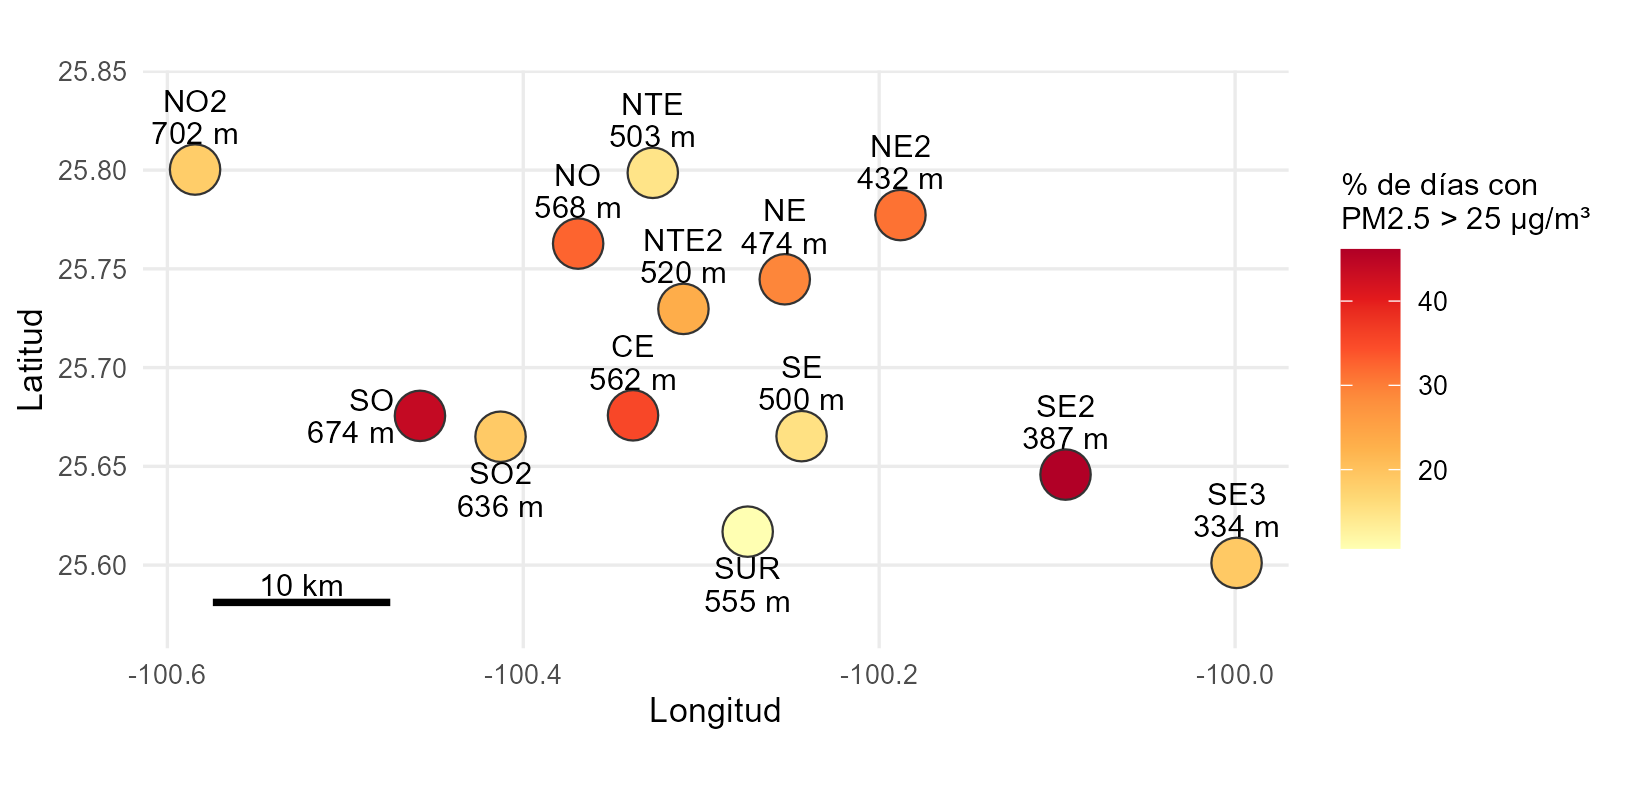
\includegraphics[width=0.70\textwidth]{figuras/mapa_estaciones_informe.png}
\caption{Estaciones de la muestra, con su altitud (m s.\,n.\,m.) y el porcentaje de días-estación con PM2.5 > 25\ugm{} en el análisis final (base v2, 2021–2025, n = 17\,828). Solo coordenadas, sin mapa base. El porcentaje de NO2 incluye el periodo con PM2.5 anómalo (Anexo~C). Elaboración propia con datos de SIMA.}
\label{fig:mapa}
\end{figure}

La Figura~\ref{fig:mapa} muestra que la superación no sigue la altitud: SO (674\,m) y SE2 (387\,m) tienen los porcentajes más altos y están en extremos opuestos del valle, mientras que SE3 (334\,m), la más baja, está por debajo de la mitad de la red. El porcentaje bajo de NO2 no sirve para este argumento: en buena parte refleja un problema de su equipo de PM2.5 (Tabla~\ref{tbl:b-cambios}).



\textbf{Contexto por estación.} SIMA describió las fuentes de las dos estaciones con más superaciones (comunicación personal, 15 de octubre de 2026), y las contrastamos con nuestros datos:
\begin{itemize}
\item \textbf{SE2 (Juárez).} Es el primer receptor de la pluma de la refinería: por la altura de los quemadores, la dispersión pasa por encima de Cadereyta (SE3) y llega a Juárez. Además, hay crecimiento urbano, vialidades sucias con resuspensión, quemas nocturnas, transporte pesado y obras viales. En nuestros datos, SE2 tiene el viento más débil de la red (1.55\,m/s de media) y el PM2.5 más ligado al PM10 (Spearman 0.82). Su cociente PM2.5/PM10 (mediana 0.40) está entre los más altos de la red (0.25 a 0.42): la fracción gruesa sigue siendo la mayor parte, pero la fina pesa relativamente más que en otras estaciones y sube en los días con superación (0.46 frente a 0.35). De forma descriptiva, en enero el PM2.5 medio de SE2 subió de 33.1 a 43.1\ugm{} entre 2023 y 2024 (19 y 30 días con dato), mientras que en SE3 no cambió (22.4\ugm); va en la misma dirección que el alza que el gobierno estatal atribuyó a la refinería, aunque sus cifras no son las nuestras (Gobierno del Estado de Nuevo León, 2024).
\item \textbf{SO (Santa Catarina).} Es una zona industrial de entrada, con suelo semidesértico, carga vehicular y receptora de la salida del viento. En nuestros datos los días con superación tienen viento más débil (diferencia de medias estandarizada de la rapidez −0.76, la mayor de la red) y un flujo del este menos intenso (\emph{u} de −1.16 frente a −2.01\,m/s). Con promedios diarios no se puede separar la acumulación local del transporte desde la ciudad.
\item \textbf{SUR (Pueblo Serena).} Su reubicación se ve en los datos: pasó de 3.0\,\% de días con superación en 2021 a 10–12\,\% desde 2022, y su presión frente a la red cambió +5.7\,mm\,Hg en la fecha de reubicación.
\end{itemize}
Son explicaciones de contexto, consistentes con los datos, que no se pueden atribuir sin inventarios de emisiones ni análisis horario de transporte.

\textbf{Cambios en la red (Tabla~\ref{tbl:b-cambios}, Anexo~B).} El PIGECA registra reubicaciones de NO (junio de 2021), SE, SO, NTE y SUR (septiembre de 2021) y NE (febrero de 2022) (SMA y CAI, 2024, p.~91); el entrenamiento excluye los días previos (D23). Los sensores de viento se renovaron en 2021 (por eso se excluye 2020) y cinco equipos de PM2.5 cambiaron en 2025. El PM2.5 de NO2 baja a la mitad del nivel de la red con su PM10 normal, y la radiación de NO2 y NTE es muy baja. Las sensibilidades a estos cambios dan mejoras de 0.079 a 0.082 (Tabla~\ref{tbl:robustez}, Anexo~C).

% ======================= 4. PREPARACIÓN =======================
\section{Preparación de la base de datos}\label{sec:preparacion}

\subsection{Datos y diagnóstico}\label{sec:datos}
SIMA entregó seis libros de Excel (2020–2025) con 87 hojas estación-año y datos horarios de 15 estaciones y 15 variables. Sobre los valores horarios esperados faltaba el 12.3\,\%. \textbf{En el PM2.5 faltaba el 26.0\,\% de las horas} (17.2\,\% en las 13 estaciones de la muestra, 2021–2025), y de esas horas el 44\,\% está en huecos de más de una semana. Los faltantes son sobre todo apagones largos: en las seis variables que se imputan o se modelan, entre el 51\,\% y el 82\,\% de las horas faltantes están en huecos de más de un día (Tabla~\ref{tbl:b-huecos}, Anexo~B). Esto descarta reconstruir esos huecos con métodos locales y motiva imputar a nivel diario con información de la red (Sección~\ref{sec:imputacion}).

\subsection{Limpieza por reglas}
Cada hora de cada variable conserva una bandera que indica si es válida o por qué se anuló; no se elimina ninguna fila (Tabla~\ref{tbl:b-limpieza}, Anexo~B). Las reglas de consistencia espacial (D14) comparan cada lectura con la mediana de la red a la misma hora (Fiebrich et al., 2010). La regla D15 anula la radiación de todo un día si su media de madrugada supera 0.02\,kW/m², y el viento que excede por mucho al de la red (Estévez et al., 2011); se agregó porque la exploración encontró radiación nocturna en NO2, SE3 y CE y vientos imposibles en SO2 y NE2. En total se invalidó el 0.7\,\% de los valores. Los extremos que pasan todas las reglas se conservan, porque pueden ser concentraciones reales. Excluimos 2020 del modelado, porque el viento cambió de nivel con la renovación de sensores de 2021 y por el confinamiento, y las estaciones NE3 y NO3, que casi no miden PM2.5. El detalle de cada regla está en el Anexo~B.

\subsection{Imputación}\label{sec:imputacion}
\textbf{Principio: la respuesta no se imputa (D18).} El PM2.5 diario se calcula solo con al menos 18 horas observadas, el criterio de suficiencia de la NOM-025-SSA1-2021. Imputar el PM2.5 crearía etiquetas de superación que nadie midió, y atiende la advertencia de SIMA sobre los huecos largos en Juárez y Santa Catarina. El costo es perder 526 días-estación con respuesta válida frente a la etapa 3. Las ventanas grandes de la meteorología se recuperan a nivel diario con la información de la red (D20); las del PM2.5 no se rellenan.



\textbf{Imputación horaria de la meteorología (D19).} Usamos los métodos de la fuente principal del curso, el paquete imputeTS (Moritz \& Bartz-Beielstein, 2017): interpolación lineal, spline y de Stineman, media móvil exponencial, filtro de Kalman, descomposición estacional y LOCF como piso. Los elegimos por enmascaramiento solo en 2021–2023: en tramos completos borramos bloques de 1 a 24\,h que sí conocemos, los imputamos con cada método y medimos el error del \textbf{promedio diario}, que es lo que entra al modelo. La regla, fijada antes de ver los resultados y corregida antes de cerrar las decisiones (registro de cambios de la fase A), descalifica los métodos cuyas imputaciones revierte la revalidación en más de 5\,\%. Exige además un error diario de a lo más el 10\,\% de la desviación de la anomalía de cada variable. La Tabla~\ref{tbl:imputacion} (Anexo~B) resume el método elegido por variable, y la Figura~\ref{fig:imputacion} (Anexo~B) muestra que en huecos de 6 a 24\,h la descomposición estacional comete cerca de la mitad del error de la interpolación lineal y que, en el PM2.5, la interpolación aplana los picos, otra razón para no imputar la respuesta. No usamos imputación por vecinos cercanos (KNN).

\textbf{Imputación diaria de la meteorología (D20).} Con la imputación horaria quedan días con una a cuatro de las ocho variables faltantes, sobre todo radiación y humedad. Para recuperarlos comparamos tres métodos en una validación por enmascaramiento con el patrón real de faltantes de 2021–2023. El primero es la mediana de las otras estaciones ese día, ajustada por la diferencia media de la estación, un método de efecto por sitio en la línea de Plaia y Bondì (2006). Los otros dos son MICE con \emph{predictive mean matching} (van Buuren \& Groothuis-Oudshoorn, 2011) y la media de estación × temporada. \textbf{En error puntual, la mediana ajustada y MICE quedan casi empatadas:} RMSE relativo medio de 0.450 frente a 0.436 si se promedian las cinco imputaciones de MICE; la mediana gana en seis de las ocho variables, incluidas temperatura y humedad, las que más faltan en 2024–2025, y MICE gana en lluvia y radiación. Una sola base de MICE tiene más error (0.593), pero eso es esperable, porque el \emph{predictive mean matching} agrega variabilidad a propósito; la media de estación × temporada queda en 0.736. Elegimos la mediana ajustada por ser determinista y simple, y usamos MICE como sensibilidad del clasificador, con 20 bases imputadas: \dauc{} = 0.078 (Tabla~\ref{tbl:robustez}). Ninguna imputación usa el PM2.5 ni la superación como predictor. Moons et al. (2006) muestran que incluir la respuesta al imputar predictores puede reducir el sesgo de las asociaciones; aquí se excluyó para conservar una evaluación predictiva en la que la respuesta de prueba no interviene en los predictores. La idea de aprovechar la red coincide con antecedentes que encontraron mejores imputaciones con información de estaciones vecinas (Quinteros et al., 2019; Belachsen \& Broday, 2022) y suficiencia de métodos simples para promedios diarios (Hadeed et al., 2020).

\textbf{Imputación de referencia del curso.} El curso recomienda como referencia de imputación con datos del SIMA el trabajo MIMA-v1 (Gómez et al., 2025; Gómez Santos et al., 2027), un modelo generativo (SAITS + CSDI) que reconstruye series horarias completas, incluidos los huecos largos. \textbf{No lo usamos porque solicitamos su dataset imputado y no obtuvimos acceso a tiempo.} El análisis natural habría sido una sensibilidad con su meteorología imputada en sus 9 estaciones (enero de 2021 a junio de 2025), conservando nuestro PM2.5 observado como respuesta, lo que es compatible con no imputar la respuesta (D18). Ese análisis tendría dos límites de alcance: su cobertura no incluye Juárez (SE2), Cadereyta (SE3), SUR ni NE2, y su PM2.5 imputado no se usaría como etiqueta. Hay coincidencias con su trabajo: en su comparación de métodos clásicos, la interpolación lineal tuvo el menor error (MAE de 4.01) y la descartaron porque suaviza los picos. Nuestro enmascaramiento confirma ese suavizado en el PM2.5; por eso no imputamos la respuesta y elegimos el método horario de la meteorología con validación. De las fuentes del curso tomamos los métodos de imputeTS (Moritz \& Bartz-Beielstein, 2017) y la validación por enmascaramiento.

\subsection{Transformaciones}
\begin{itemize}
\item \textbf{Agregado diario:} un valor diario existe con al menos 18 horas válidas de esa variable.
\item \textbf{Viento:} componentes \emph{u} (este-oeste) y \emph{v} (norte-sur) y rapidez, porque la dirección es circular.
\item \textbf{Lluvia:} horas con lluvia en el día, porque la unidad de la cantidad no está confirmada.
\item \textbf{Presión:} anomalía respecto de la media de su sitio en el entrenamiento (D17); separa la altitud (medias de 700.8 a 731.5\,mm\,Hg) del efecto meteorológico.
\item \textbf{Escalado:} todas las variables se estandarizan con medias y desviaciones del entrenamiento.
\item \textbf{Sin logaritmos (D16):} en la validación progresiva, transformar la lluvia y el viento solo subió el AUC 0.003 y 0.007, y el logaritmo sobrecorregía la asimetría del viento (de +0.37 a −0.98).
\end{itemize}

\subsection{Muestra final, exclusiones y posible sesgo}\label{sec:muestra}
La Tabla~\ref{tbl:exclusiones} clasifica los 23\,738 días-estación posibles (13 estaciones × 1\,826 días) según su causa de exclusión: la imputación diaria recupera los días con una a cuatro meteorológicas faltantes, no los que tienen cinco o más, y el entrenamiento excluye los días previos a cada reubicación (D23), porque corresponden a otro sitio. El análisis final queda con \textbf{17\,828 días-estación}: 10\,965 de entrenamiento (2021–2023; 25.9\,\% de superación) y 6\,863 de prueba (2024–2025; 26.2\,\%). Frente a la etapa 3 hay 2\,438 días más, sobre todo en García (NO2: de 511 a 1\,532), donde faltaba la radiación, y en Escobedo (NTE: de 597 a 1\,373), donde faltaba la humedad (Anexo~C). En la prueba, el 27\,\% de los días (1\,876 de 6\,863) tiene al menos una variable meteorológica completada con la mediana de la red, sobre todo en NTE (646 de 662) y NE (452 de 657). No es una fuga de información, porque la imputación no usa la respuesta, pero conviene tenerlo presente: sin imputación diaria la mejora es de 0.071 (Tabla~\ref{tbl:faltantes}).

\begin{table}[!htbp]
\centering\small
\caption{Causas de exclusión de los 23\,738 días-estación posibles (2021–2025) y respuesta de cada grupo donde existe. Las causas (a) a (d) suman el total; (e) es parte de (b) y (c). Detalle por estación, temporada y año en el Anexo~B.}
\label{tbl:exclusiones}
\begin{tabularx}{\textwidth}{Lrrcrrr}
\toprule
Grupo & Días-estación & \% & ¿En el análisis? & \% superación & Mediana de PM2.5 & \% con PM2.5 > 40\\
\midrule
(a) Sin PM2.5 suficiente (< 18\,h observadas) & 4\,346 & 18.3 & No & — & — & —\\
(b) Respuesta y meteorología completa & 15\,011 & 63.2 & Sí & 27.0 & 18.5 & 5.5\\
(c) Respuesta y 1–4 meteorológicas imputadas & 4\,192 & 17.7 & Sí & 23.5 & 17.7 & 3.7\\
(d) Respuesta y 5–8 meteorológicas faltantes & 189 & 0.8 & No & 33.3 & 18.7 & 5.8\\
(e) De (b) o (c), previos a una reubicación & 1\,375 & 5.8 & No & 29.5 & 19.2 & 4.3\\
\bottomrule
\end{tabularx}
\end{table}

Donde hay respuesta, los excluidos se parecen a los incluidos: 33.3\,\% de superación en (d), con solo 189 días, y 29.5\,\% en (e), frente a 27.0\,\% en (b). Los días que recupera la imputación (c) tienen menos superación en promedio (23.5\,\%), pero la diferencia cambia de signo según la estación: en NO2, donde faltaba la radiación, es de 22.7\,\% en (c) y 9.8\,\% en (b). Con casos completos, la etapa 3 daba a NO2 10.0\,\% de superación y la base final 18.4\,\%: esa exclusión sesgaba la muestra. Los días sin PM2.5 suficiente (a) se concentran en NO (57\,\% de sus días, con un hueco de 532 días desde marzo de 2024), NE2 (33\,\%) y SUR (26\,\%), y en 2024–2025 (24\,\% y 30\,\%, frente a 10–15\,\% antes); la mitad están en huecos de más de una semana y se reparten casi igual entre temporadas. Su PM10, disponible en el 86\,\% de ellos, es menor que el de los días con respuesta en 31 de 39 combinaciones de estación y temporada, así que no parecen concentrarse en días de contaminación alta. Aun así, no podemos descartar un sesgo por datos faltantes, sobre todo en la prueba y en NO y NE2. La Tabla~\ref{tbl:faltantes} resume qué se imputó, qué se excluyó y qué mostraron las sensibilidades.

\begin{table}[!htbp]
\centering\small
\caption{Resumen del tratamiento de los datos faltantes: qué se imputó, qué se excluyó y qué mostró el análisis de sensibilidad (\dauc{} de M1 frente a M0 con LDA en la prueba; análisis final: 0.079 [0.054, 0.104]).}
\label{tbl:faltantes}
\begin{tabularx}{\textwidth}{>{\raggedright\arraybackslash}p{2.1cm}LL}
\toprule
Tratamiento & Qué datos & Sensibilidad (\dauc{} [IC 95\,\%])\\
\midrule
Se imputó & Meteorología horaria en huecos cortos (2 a 12\,h según la variable; Tabla~\ref{tbl:imputacion}, Anexo~B) y meteorología diaria de los días con 1–4 de 8 variables faltantes (4\,192 días-estación) & Sin imputación diaria (casos completos): 0.071 [0.047, 0.096]; con MICE (m = 20): 0.078 [0.055, 0.103]; imputación diaria solo con ≤ 2 faltantes: 0.077 [0.052, 0.102]\\
No se imputó & PM2.5 (la respuesta): solo se usa con ≥ 18\,h observadas & PM2.5 interpolado en huecos ≤ 3\,h: 0.079 [0.053, 0.105]\\
Se excluyó & (a) días sin PM2.5 suficiente (4\,346), (d) días con 5–8 meteorológicas faltantes (189) y (e) días previos a una reubicación (1\,375, solo en el entrenamiento) & Reubicaciones según SIMA: 0.081 [0.054, 0.107]; los excluidos con respuesta tienen una superación parecida a los incluidos (Tabla~\ref{tbl:exclusiones})\\
\bottomrule
\end{tabularx}
\end{table}

% ======================= 5. MODELACIÓN =======================
\section{Modelación y validación}\label{sec:modelacion}

\subsection{Ruta de análisis}\label{sec:ruta}
La Tabla~\ref{tbl:ruta} vincula cada técnica con su pregunta, sus variables, su respaldo metodológico y artículos que la aplicaron en contextos ambientales o con series de tiempo. Para nuestro objetivo, el PCA muestra qué condiciones meteorológicas varían juntas. El LDA, fijado en el protocolo, mide cuánto separa la meteorología los días con y sin superación por encima de estación y temporada. La logística responde lo mismo sin suponer normalidad y expresa cada efecto en momios. El bootstrap por bloques da un intervalo que respeta la persistencia entre días y estaciones. La validación progresiva comprueba que la mejora se repite en años que el modelo no vio.

\begin{table}[!htbp]
\centering\footnotesize
\caption{Ruta de análisis: técnica y tipo, pregunta, variables, justificación, respaldo metodológico y aplicación previa en contextos ambientales o de series de tiempo.}
\label{tbl:ruta}
\begin{tabularx}{\textwidth}{>{\raggedright\arraybackslash}p{2.3cm}>{\raggedright\arraybackslash}p{2.5cm}>{\raggedright\arraybackslash}p{2.2cm}L>{\raggedright\arraybackslash}p{2.0cm}L}
\toprule
Técnica & Pregunta & Variables & Por qué es adecuada & Respaldo & Aplicación previa\\
\midrule
Componentes principales (PCA; interdependencia) & ¿Cómo se estructura la correlación de la meteorología? & 8 meteorológicas, como anomalías por estación & Resume variables correlacionadas en pocos ejes; describe, no predice & Jolliffe y Cadima (2016) & Ramírez-Velarde et al. (2024): meteorología de la ZMM y contingencias; Mohd Shafi'i y Juahir (2024): 8 estaciones de Malasia\\
LDA (dependencia, fijada en el protocolo) & ¿Cuánto mejora M1 a M0? & Estación y temporada; en M1, + 8 meteorológicas & Función lineal interpretable; con la misma partición, M1 − M0 se atribuye a la meteorología & Johnson y Wichern (2007); Krzanowski (1975) & Mohd Shafi'i y Juahir (2024): 90.5\,\% de los casos bien asignados a grupos de estaciones por contaminación\\
Regresión logística (dependencia, en paralelo) & ¿Qué variables influyen? ¿Depende la conclusión de los supuestos del LDA? & Las mismas que el LDA & No supone normalidad ni covarianzas iguales; referencia para interpretar las variables & Efron (1975); James et al. (2021) & Vélez-Pereira et al. (2025): superaciones diarias de PM2.5 y PM10 en Chile; Saminathan y Malathy (2023): PM2.5 con meteorología en Pekín\\
Bootstrap pareado por bloques & ¿Qué tan incierta es la \dauc? & Predicciones de la prueba en bloques de 14 días & La contaminación alta persiste días y afecta a varias estaciones & Carlstein (1986); Künsch (1989) & Wilks (2019): datos atmosféricos autocorrelacionados\\
Validación temporal progresiva & ¿Se sostiene la mejora en años posteriores? & Entrenar en años anteriores y evaluar el siguiente & Con datos ordenados en el tiempo, la validación aleatoria sobreestima el desempeño & Roberts et al. (2017) & Roberts et al. (2017): datos ecológicos con estructura temporal\\
\bottomrule
\end{tabularx}
\end{table}

\subsection{Componentes principales}\label{sec:pca-metodo}
El PCA se ajustó solo con el entrenamiento, sobre las anomalías de cada variable respecto de la media de su estación, para que los ejes describan la variación meteorológica y no las diferencias entre sitios. La adecuación es modesta: KMO = 0.64, valor que Kaiser y Rice (1974) clasifican como mediocre; por ello el PCA se utiliza con fines exploratorios. La prueba de Bartlett (1950) rechaza la esfericidad (χ² = 26\,503, gl = 28, p < 0.001). Tres valores propios superan 1 (criterio de Kaiser, 1960) y explican el 66.5\,\% de la varianza. \textbf{Ese 66.5\,\% es la parte de la variación conjunta de las ocho variables meteorológicas que resumen los tres ejes; no significa que la meteorología explique el 66.5\,\% de las superaciones.} Tampoco es un predictor: maximizar la varianza no maximiza la separación entre clases, y su primer eje mezcla variables que se asocian con la superación en sentidos contrarios (Sección~\ref{sec:coef}). En la etapa 3, usar los tres componentes en lugar de las ocho variables dio una mejora menor (Anexo~A). \textbf{El PCA resume la correlación entre variables, pero no elimina la autocorrelación temporal de los días.}

\subsection{LDA y el tratamiento de estación y temporada}\label{sec:lda}
\textbf{Codificación.} Estación (13 niveles) y temporada (3) entran como variables indicadoras, \emph{k} − 1 por factor, con categoría de referencia CE (Obispado) y temporada cálida-húmeda: 12 indicadoras de estación y 2 de temporada, estandarizadas con el entrenamiento como el resto de los predictores. \textbf{M0} usa solo esas 14 indicadoras. Su función discriminante asigna a cada día un puntaje que es la suma de un efecto de estación y uno de temporada, así que M0 da una misma probabilidad a todos los días de cada una de las 39 combinaciones estación × temporada: es la referencia de lo que ya se sabe sin la meteorología diaria. \textbf{M1} agrega a las mismas indicadoras las ocho variables meteorológicas continuas (22 predictores).

\textbf{Por qué es apropiado para los dos modelos.}
\begin{enumerate}
\item Mismo método y misma partición: la diferencia M1 − M0 se atribuye a la meteorología y no al clasificador.
\item El criterio de Fisher, que busca la combinación lineal que separa las medias de las clases en relación con la dispersión dentro de ellas, no requiere normalidad. La regla y sus probabilidades solo son óptimas si los predictores son normales con una covarianza común en las dos clases (Johnson \& Wichern, 2007).
\item Con indicadoras, la normalidad multivariada no se cumple literalmente. Por eso el LDA se usa como clasificador lineal y no como modelo generativo bien especificado. Para predictores mixtos, Krzanowski (1975) propuso el modelo de localización, que generaliza el discriminante a variables binarias y continuas; la regla lineal que usamos es una aproximación que supone que el efecto de la meteorología sobre la separación es el mismo en todas las estaciones y temporadas.
\item El logit de la probabilidad posterior del LDA es lineal en los predictores, igual que en la regresión logística. Con normalidad condicional y covarianza común, el LDA puede ser más eficiente asintóticamente que la logística (Efron, 1975). La logística no exige una distribución normal de los predictores, aunque sí especifica una forma para la probabilidad condicional; su comparación con el LDA aporta aquí evidencia empírica de estabilidad.
\end{enumerate}

\textbf{Dos clasificadores en paralelo.} Conservamos el LDA, fijado en el protocolo antes de evaluar, y reportamos junto a él la regresión logística con los mismos predictores, que da resultados similares y es la referencia para interpretar las variables (Sección~\ref{sec:logistica}). Tampoco resuelve todo: requiere especificar bien la relación de cada predictor con el logit (razón 4), y la autocorrelación invalida su inferencia convencional.

\textbf{Prior y corte.} La probabilidad previa es la prevalencia del entrenamiento (0.259), y un día se clasifica como superación si su probabilidad posterior es al menos esa prevalencia. El corte se fijó antes de ver la prueba; la Sección~\ref{sec:umbral} evalúa cortes elegidos con el entrenamiento para usos concretos.

\subsection{Supuestos: qué se revisó, qué implica y qué no se puede concluir}\label{sec:supuestos}

\begin{table}[!htbp]
\centering\footnotesize
\caption{Supuestos del LDA y un diagnóstico adicional de los residuos, revisados en el entrenamiento (n = 10\,965) y en los errores de la prueba (n = 6\,863), con su implicación y su tratamiento (base v2).}
\label{tbl:supuestos}
\begin{tabularx}{\textwidth}{>{\raggedright\arraybackslash}p{2.45cm}>{\raggedright\arraybackslash}p{2.7cm}LLL}
\toprule
Supuesto & Diagnóstico & Resultado & Implicación & Cómo se tomó en cuenta\\
\midrule
Normalidad multivariada por clase & Mardia (1970), 8 meteorológicas; las indicadoras son discretas & No se cumple: asimetría χ² = 99\,015 y 198\,072 (gl = 120, p < 0.001); lluvia con asimetría de 7.6 y 19.9 & No está garantizada la optimalidad de la regla ni la calibración de sus probabilidades & LDA como clasificador; logística como contraste (0.071)\\
Igualdad de covarianzas & M de Box (1949) y razón de desviaciones por clase & No se cumple: χ² = 3\,213 (gl = 36, p < 0.001); diferencia sobre todo en la lluvia (razón 0.40) y en \emph{v} (0.78); en las demás, 0.85–1.05 & La igualdad de covarianzas no está respaldada; una frontera lineal puede perder eficiencia & QDA como alternativa: no mejora (0.788 frente a 0.792)\\
Independencia & ACF del residuo dentro de cada estación; correlación entre estaciones el mismo día & No se cumple: ACF a 1 día de 0.42 en el residuo de M1 (0.50 en la respuesta); 0.36 entre estaciones & Los errores estándar usuales no valen & Bootstrap por bloques; estabilidad por bootstrap; sin valores p\\
Multicolinealidad & VIF y número de condición & Baja: VIF máximo 2.28 (temperatura); número de condición 2.97 & Los coeficientes se pueden leer en conjunto & Presión como anomalía; interpretación conjunta\\
Diagnóstico adicional: variación de los residuos y calibración & Varianza de Y − \^{p} por temporada y estación (Brown-Forsythe, solo descriptivo por la dependencia); error por decil & La varianza de Y − \^{p} cambia entre temporadas (0.086–0.205; F = 503); en el decil más alto el error es 1.34 veces el esperado; pendiente de recalibración de 0.82 & Esperable en parte por la respuesta binaria; no es un supuesto incumplido del LDA & Las probabilidades necesitan recalibración antes de comunicarse como riesgos; se usan como puntajes\\
\bottomrule
\end{tabularx}
\end{table}

La Tabla~\ref{tbl:supuestos} muestra que el LDA no cumple sus supuestos distribucionales, y conviene precisar qué hace cada herramienta. El bootstrap por bloques estima la incertidumbre del \textbf{desempeño} respetando grupos de fechas, pero no vuelve independientes los datos con los que se ajusta el LDA: por eso no reportamos valores p de los coeficientes. El PCA controla la correlación entre variables, no la autocorrelación. La validación temporal mide cómo clasifica el modelo en años posteriores, aunque 2024–2025 ya se habían usado en una prueba de viabilidad preliminar (4 de octubre), en la evaluación de la etapa 3 y en la de la etapa 4. En las etapas 3 y 4 las decisiones se cerraron antes de evaluar la prueba con la base correspondiente; sin embargo, los cambios de la etapa 4 se decidieron después de conocer el resultado de la etapa 3. La mejora coincide con la de la validación progresiva dentro del entrenamiento (Sección~\ref{sec:validacion}), pero esa prueba ya no es completamente nueva y lo declaramos. Por todo esto, la evidencia que presentamos es empírica: validación temporal, comparación con la logística y estabilidad de los coeficientes. No interpretamos la función discriminante como un modelo generativo.

\subsection{Regresión logística: variables y linealidad}\label{sec:logistica}
\textbf{Variables relevantes.} Ajustamos M1 logístico con los 22 predictores estandarizados del LDA, con intervalos del mismo bootstrap por bloques del entrenamiento y sin valores p, que la dependencia entre días invalida. Las ocho meteorológicas tienen el signo del LDA (Figura~\ref{fig:coef}, panel b). Con lo demás constante, 1 DE más de rapidez del viento (0.85\,m/s) multiplica las momios de superación por 0.49 (IC 95\,\% [0.39, 0.62]); de presión respecto de lo normal del sitio (3.5\,mm\,Hg), por 0.58 [0.49, 0.70]; de temperatura (6.3\,°C), por 1.78 [1.24, 2.71]; de horas de lluvia (1.1\,h), por 0.81 [0.64, 0.93], y de radiación (0.08\,kW/m²), por 0.82 [0.67, 1.00], cuyo intervalo llega a 1, así que su efecto es débil. La humedad, \emph{u} y \emph{v} no tienen signo estable. Al permutar cada grupo de variables en la prueba, el AUC cae sobre todo con la temporada (0.138) y la estación (0.067); entre las meteorológicas, la caída se concentra en la presión, la rapidez del viento y la temperatura (0.03 a 0.05 cada una), y las demás lo mueven menos de 0.01. Como esas tres variables están correlacionadas, la permutación no permite ordenarlas entre sí: \textbf{la mejora de M1 descansa en el grupo ventilación–presión–temperatura}, con los dos clasificadores.

\textbf{Linealidad en la escala logit (Figura~\ref{fig:linealidad}, Anexo~C).} En el entrenamiento, los logits empíricos por deciles, ajustados por las demás variables, y un modelo aditivo generalizado (GAM) logístico con un spline penalizado por variable (Wood, 2017) muestran curvatura: de 5.4 a 8.4 grados de libertad efectivos, salvo en la lluvia (1.6); con días autocorrelacionados, esos grados de libertad pueden estar inflados. El efecto de la temperatura crece más rápido arriba de 28\,°C, el de la rapidez del viento se aplana arriba de 3\,m/s y el de la humedad cae arriba de 70\,\%; la presión es casi lineal. La regla fijada antes de evaluar la prueba (splines si suben el AUC de validación en ≥ 0.005 en los dos pliegues) se cumplió (+0.006 en 2022 y +0.021 en 2023), así que los reportamos como tratamiento de la no linealidad: en la prueba, M1 con splines llega a un AUC de 0.811 y mejora a M0 logístico en 0.090 [0.060, 0.120], frente a 0.071 con la forma lineal. El modelo principal no cambia; su forma lineal, si acaso, subestima lo que aporta la meteorología. La indicadora «llovió» no agrega nada a las horas de lluvia.

\subsection{Análisis de los errores}\label{sec:errores}
Con las predicciones de la prueba calculamos el residuo de cada día (superación observada menos probabilidad) y su autocorrelación dentro de cada estación (Figura~\ref{fig:acf}).

\begin{figure}[!htbp]
\centering
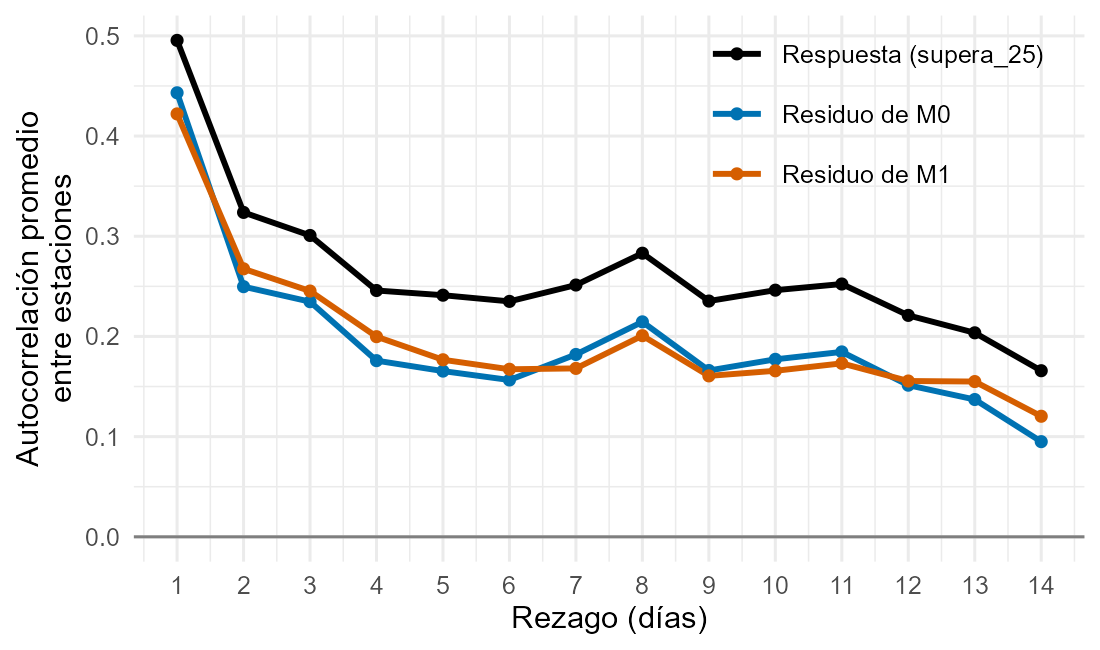
\includegraphics[width=0.46\textwidth]{figuras/acf_residuos_informe.png}
\caption{Autocorrelación promedio entre estaciones de la respuesta y de los residuos de M0 y M1, a rezagos de 1 a 14 días, dentro de cada estación (prueba 2024–2025, n = 6\,863).}
\label{fig:acf}
\end{figure}

La Figura~\ref{fig:acf} muestra que agregar la meteorología reduce poco la dependencia. La autocorrelación a un día baja de 0.50 en la respuesta a 0.44 con M0 y a 0.42 con M1, y la correlación entre estaciones el mismo día baja de 0.48 a 0.36. \textbf{El modelo no absorbe toda la dependencia}, y esa es la razón del bootstrap por bloques y del límite a la interpretación. La varianza de los errores también difiere entre temporadas y estaciones, algo esperable en parte con una respuesta binaria, y la calibración es imperfecta: la pendiente de la recalibración es 0.82, cuando el ideal es 1, y en todas las temporadas queda entre 0.69 y 0.76 (Anexo~C). Las probabilidades deben leerse como puntajes.

\subsection{Validación}\label{sec:validacion}
La métrica principal es el AUC en la prueba: la probabilidad de que un día con superación reciba un puntaje mayor que uno sin superación, no un porcentaje de aciertos (Fawcett, 2006). La complementan la exactitud balanceada, la sensibilidad, la especificidad, el puntaje de Brier (Brier, 1950) y la calibración.

\textbf{Bootstrap por bloques.} Remuestreamos bloques de 14 días consecutivos con todas las estaciones, manteniendo fijas las predicciones (1\,000 réplicas; Carlstein, 1986; Künsch, 1989); también lo hicimos estratificado por temporada, con cada bloque en la temporada de la mayoría de sus días (22 de lluvias, 14 de seca-cálida y 17 de seca-fría). \textbf{Los 14 días son el tamaño de cada bloque del remuestreo, no un horizonte de pronóstico:} el modelo clasifica cada día con la meteorología de ese mismo día, y los bloques solo mantienen juntos los días cercanos, que se parecen, para no subestimar la incertidumbre. No elimina la autocorrelación de los datos ni la incorpora al ajuste del LDA o de la logística: es una validación temporal útil, no una confirmación independiente. Remuestrear días sueltos subestimaría la incertidumbre; a 14 días, la autocorrelación del residuo de M1 baja a 0.12 (Figura~\ref{fig:acf}), que todavía no es cero, así que el intervalo con bloques de 28 días, [0.045, 0.110], es la versión conservadora y tampoco incluye el cero. Estratificado, el IC 95\,\% de \dauc{} es [0.056, 0.101] con LDA y [0.050, 0.091] con logística, casi igual que sin estratificar ([0.054, 0.104] y [0.047, 0.095]; Tabla~\ref{tbl:robustez}, Anexo~C). Los intervalos se condicionan a la preparación elegida y no incorporan toda la incertidumbre de limpieza, selección e imputación; en MICE se agruparon 20 × 200 réplicas sin evaluar la cobertura de ese procedimiento.

\textbf{Validación progresiva y etapa 3.} Con la base final, la mejora fue de 0.074 al validar 2022 y de 0.083 al validar 2023. Estos pliegues diagnostican la estabilidad del ajuste: la imputación y su selección usaron todo 2021–2023, y validar todo el procedimiento requeriría repetirlas dentro de cada pliegue. De la etapa 3 a la 4, la mejora pasó de 0.070 a 0.079 (Tabla~\ref{tbl:puente}, Anexo~C): no imputar la respuesta y cambiar la imputación horaria casi no la mueve (0.074), la imputación diaria la sube a 0.081 porque M0 clasifica peor en la muestra ampliada, y quitar los días previos a las reubicaciones la deja en 0.079.

\subsection{Técnicas no exitosas o no adoptadas}
El Anexo~A resume, con su resultado, las técnicas probadas o consideradas que no se adoptaron: conglomerados (etapa 1), componentes principales como predictores (\dauc{} 0.064), interacción estación × temporada (0.056), logaritmos, QDA (AUC 0.788 frente a 0.792), MICE (sensibilidad, 0.078), MIMA-v1 y vecinos cercanos. Las alternativas evaluadas numéricamente conservaron la conclusión principal. Para las técnicas consideradas pero no ejecutadas, incluido MIMA-v1, no se dispone de una comparación de desempeño.

% ======================= 6. RESULTADOS =======================
\section{Resultados}\label{sec:resultados}

\subsection{Desempeño de M0 y M1}\label{sec:desempeno}

\begin{figure}[!htbp]
\centering
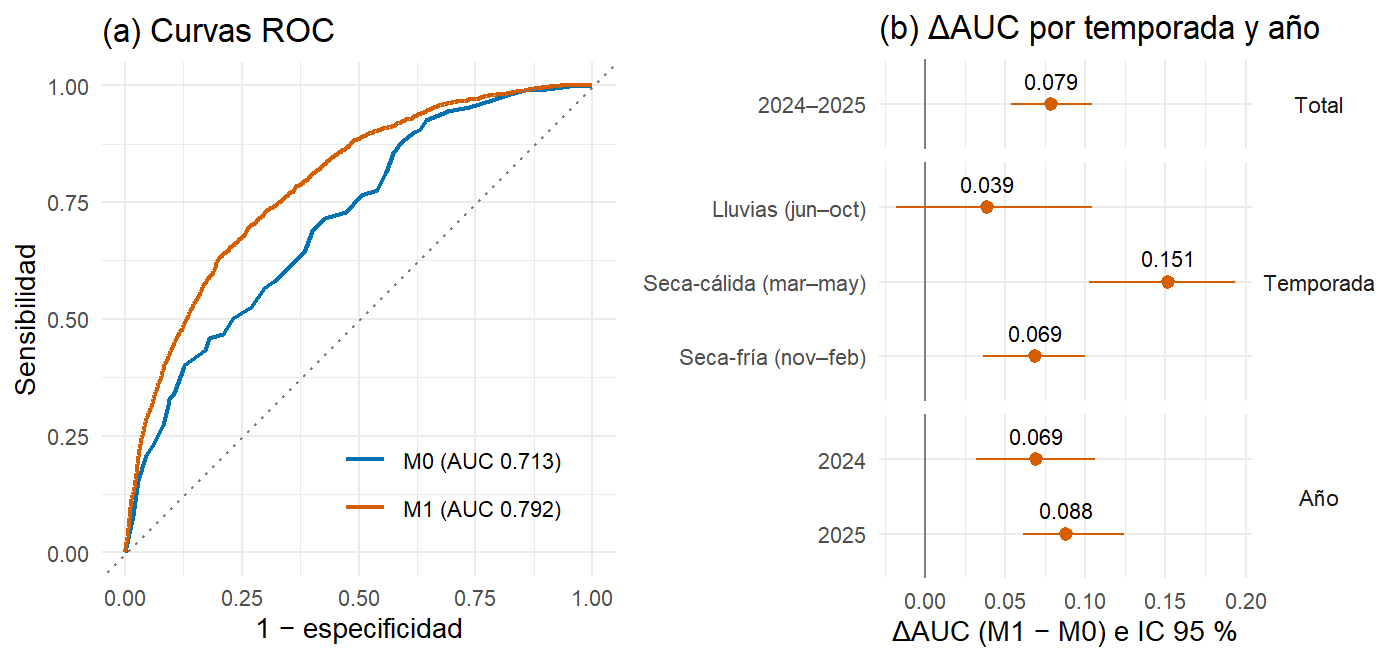
\includegraphics[width=0.64\textwidth]{figuras/roc_y_dauc_informe.png}
\caption{(a) Curvas ROC de M0 y M1 y (b) \dauc{} en total, por temporada y por año, con IC 95\,\% por bootstrap pareado por bloques de 14 días (LDA; prueba 2024–2025, análisis final, n = 6\,863).}
\label{fig:roc}
\end{figure}

\begin{table}[!htbp]
\centering\small
\caption{Desempeño de los dos clasificadores en la prueba 2024–2025 (análisis final, n = 6\,863; 26.2\,\% de superación; corte 0.259). Diferencia M1 − M0 con IC 95\,\% por bootstrap pareado por bloques de 14 días.}
\label{tbl:metricas}
\begin{tabularx}{\textwidth}{>{\raggedright\arraybackslash}p{2.6cm}rrCrrC}
\toprule
Métrica & LDA M0 & LDA M1 & LDA M1 − M0 [IC 95\,\%] & Log. M0 & Log. M1 & Logística M1 − M0 [IC 95\,\%]\\
\midrule
AUC & 0.713 & 0.792 & \textbf{0.079} [0.054, 0.104] & 0.721 & 0.792 & \textbf{0.071} [0.047, 0.095]\\
Exactitud balanceada & 0.634 & 0.711 & 0.077 [0.051, 0.100] & 0.631 & 0.711 & 0.080 [0.054, 0.103]\\
Sensibilidad & 0.565 & 0.742 & 0.177 & 0.580 & 0.739 & 0.158\\
Especificidad & 0.703 & 0.680 & −0.023 & 0.682 & 0.684 & 0.002\\
Puntaje de Brier & 0.172 & 0.154 & −0.018 & 0.170 & 0.153 & −0.017\\
\bottomrule
\end{tabularx}
\end{table}

\textbf{La meteorología del día mejora el AUC entre 0.071 (regresión logística) y 0.079 (LDA) sobre estación y temporada, en la clasificación retrospectiva de 2024–2025} (Tabla~\ref{tbl:metricas}). Estación y temporada ya separan buena parte de los días con superación (AUC de 0.713 con LDA y 0.721 con logística); con la meteorología, los dos llegan a 0.792, y ningún intervalo de la diferencia incluye el cero. M1 detecta el 74\,\% de los días con superación, contra el 56\,\% (LDA) o el 58\,\% (logística) de M0, con una especificidad parecida (LDA: de 0.70 a 0.68; logística: 0.68 en los dos), y el Brier baja. La curva ROC de M1 queda por encima de la de M0 en casi todo el rango (Figura~\ref{fig:roc}, panel a).

\textbf{Por temporada (Figura~\ref{fig:roc}, panel b).} La mejora sobre M0 es mayor en seca-cálida, de marzo a mayo (\dauc{} 0.151 [0.102, 0.193]). En esa temporada la estación separa poco los días (AUC de M0 de 0.58, frente a 0.67–0.68 en las otras dos), así que la meteorología tiene más espacio para aportar. En seca-fría la mejora es de 0.069 [0.037, 0.100]. En la temporada de lluvias es 0.039 (IC 95\,\% [−0.018, 0.104]); este intervalo no permite establecer una ganancia adicional respecto de M0. En esa temporada la superación ocurre en el 9.7\,\% de los días, y el resultado no demuestra ausencia de capacidad discriminante: el AUC de M1 es aproximadamente 0.706. El orden entre temporadas es descriptivo y se refiere a la mejora sobre M0; frente a la persistencia el orden cambia (Sección~\ref{sec:persistencia}). \textbf{Por año}, la mejora es de 0.069 [0.032, 0.106] en 2024 y de 0.088 [0.061, 0.124] en 2025.

\textbf{Días-estación y episodios.} Un episodio es una racha de días consecutivos con superación en una estación; un día sin dato la corta. Los 1\,799 días-estación con superación de la prueba forman 733 episodios (mediana de 2 días y máximo de 16; el 47\,\% dura un solo día). M1 marca al menos un día del 72\,\% de los episodios y el primer día del 66\,\% (M0: 49\,\% en los dos casos); de las 219 rachas que forman los 349 días-estación con PM2.5 > 40\ugm, marca al menos un día del 90\,\% (M0: 77\,\%). Según la magnitud (Figura~\ref{fig:magnitud}, Anexo~C), M1 marca el 90\,\% de los días-estación con PM2.5 > 40\ugm{} (M0: 81\,\%) y el 21\,\% de los que tienen menos de 15\ugm{} (M0: 27\,\%); los errores se concentran cerca de 25\ugm.

\subsection{Estructura de la meteorología (PCA)}\label{sec:pca}
La Figura~\ref{fig:pca} muestra las cargas de los tres componentes, que juntos resumen el 66.5\,\% de la variación de las ocho variables meteorológicas (no de las superaciones). El primero (36\,\%) es un \textbf{día cálido, soleado y ventilado}, con temperatura, radiación y rapidez del viento positivas, y presión y \emph{u} negativas (más flujo del este). El segundo (17\,\%) es un \textbf{día húmedo y lluvioso}, con humedad, lluvia y \emph{v} positivas y \emph{u} negativa. El tercero (13\,\%) es un \textbf{día de presión baja y poco viento}.

\begin{figure}[!htbp]
\centering
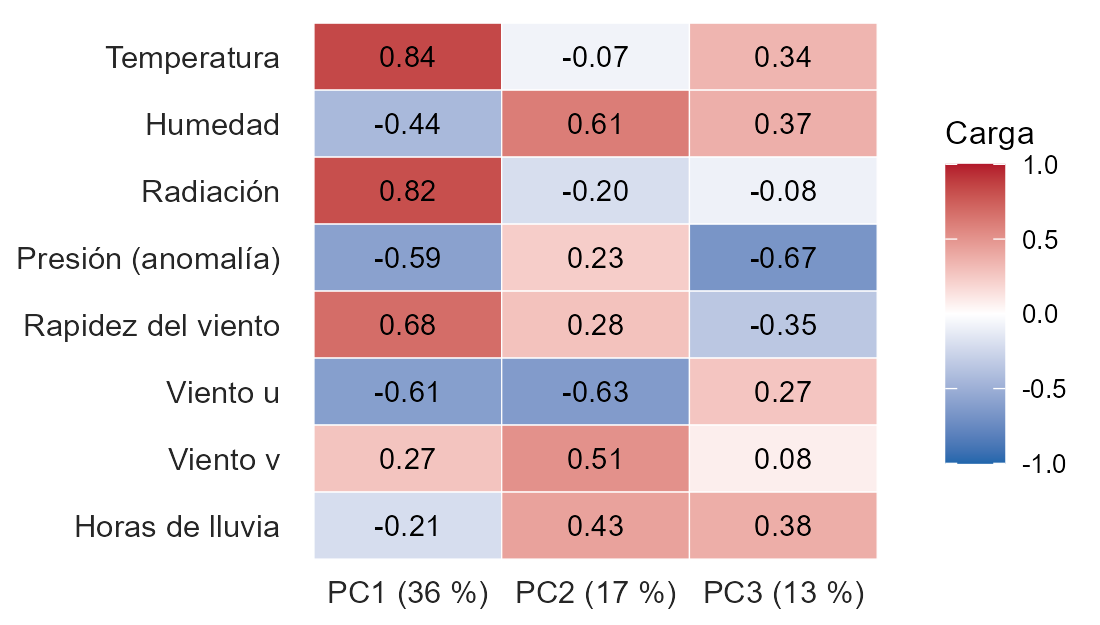
\includegraphics[width=0.46\textwidth]{figuras/pca_cargas_informe.png}
\caption{Cargas de los tres primeros componentes principales (anomalías por estación; entrenamiento 2021–2023 del análisis final, n = 10\,965). Entre paréntesis, el porcentaje de varianza de las ocho variables meteorológicas que explica cada componente.}
\label{fig:pca}
\end{figure}

\subsection{Coeficientes del LDA y de la logística}\label{sec:coef}
Solo interpretamos los coeficientes cuyo signo se mantiene en al menos el 95\,\% de 1\,000 réplicas del bootstrap por bloques en el entrenamiento (Figura~\ref{fig:coef}). Con signo estable, y condicional a las demás variables, la superación se asocia con \textbf{menor rapidez del viento} (−0.50 [−0.63, −0.35]), \textbf{presión más baja de lo normal para el sitio} (−0.46 [−0.57, −0.30]) y \textbf{mayor temperatura} (0.44 [0.16, 0.70]), y en menor medida con menos horas de lluvia y menos radiación. La temperatura tiene una correlación de estructura casi nula (−0.07), es decir, poca correlación marginal con el puntaje discriminante, aunque su coeficiente es positivo al ajustar por estación, temporada y las demás variables; estas correlaciones no sustituyen a los coeficientes condicionales (Rencher, 1992), y no interpretamos ese coeficiente común como una demostración separada para cada temporada. Por eso el primer componente, que junta temperatura y viento, mezcla efectos opuestos. Las ocho variables meteorológicas tienen el mismo signo en el LDA y en la logística (panel b; Sección~\ref{sec:logistica}), y las cinco de signo estable lo conservan en los pliegues que validan 2022 y 2023. \textbf{No interpretamos la humedad ni las componentes \emph{u} y \emph{v},} cuyo signo no es estable, ni ordenamos las variables por el tamaño de su coeficiente.

Dos signos piden cautela. \textbf{Radiación:} sin ajustar, dentro de cada temporada, se asocia ligeramente con más superación (correlación de +0.06 a +0.11), y el signo negativo solo aparece al ajustar; además, las partículas reducen la radiación que llega a la superficie, así que la relación puede ir del PM2.5 a la radiación, y no la interpretamos como efecto. \textbf{Presión:} la asociación con presión baja aparece también sin ajustar dentro de cada temporada (correlación de −0.20 a −0.30), así que no es un artefacto del modelo, pero va en contra de la explicación más común, que liga la acumulación con sistemas de alta presión. En nuestros datos la anomalía de presión baja acompaña al aire más cálido (correlación de −0.52 a −0.68 con la temperatura), y una explicación posible son situaciones previas al paso de frentes; es una hipótesis sin respaldo en este análisis, que requiere datos sinópticos.

\begin{figure}[!htbp]
\centering
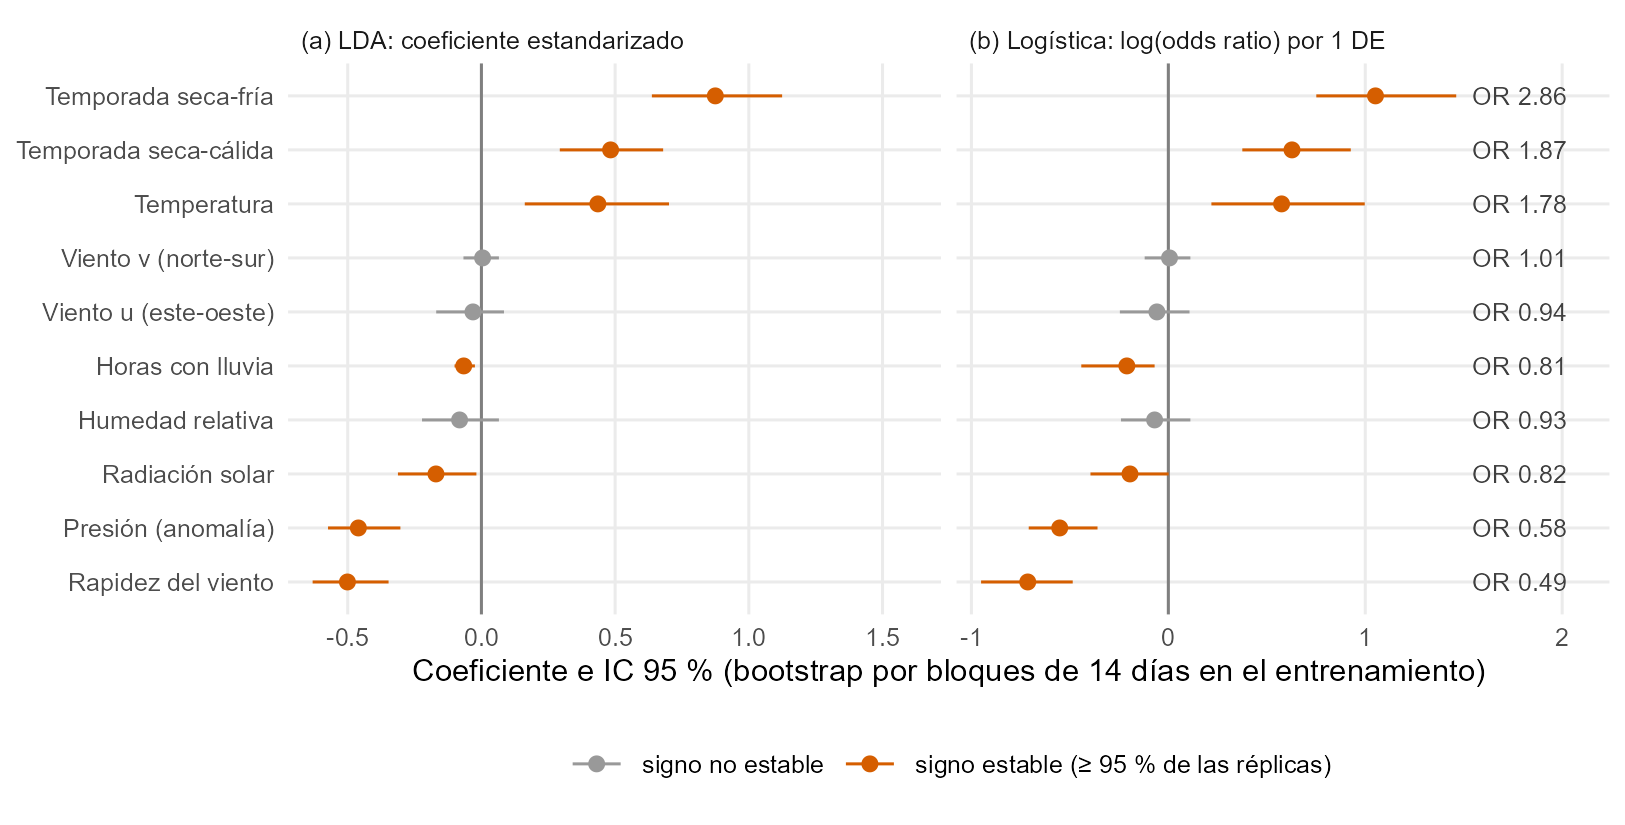
\includegraphics[width=0.68\textwidth]{figuras/coef_lda_logistica_informe.png}
\caption{Coeficientes de la meteorología y la temporada en M1: (a) LDA, coeficiente estandarizado; (b) regresión logística, logaritmo del odds ratio (OR) por 1 DE, con el OR a la derecha. IC 95\,\% por bootstrap por bloques de 14 días en el entrenamiento (1\,000 réplicas, n = 10\,965). En color, los de signo estable; la radiación lo es, pero su intervalo en la logística llega a 1, así que su efecto es débil. Las indicadoras de estación están en el Anexo~C.}
\label{fig:coef}
\end{figure}

\subsection{Robustez y sensibilidades}\label{sec:robustez}
La mejora se mantiene entre 0.071 y 0.082 en todas las variantes de preparación y validación, y ningún intervalo incluye el cero (Tabla~\ref{tbl:robustez}, Anexo~C): logística, MICE (0.078), bloques de 7 y 28 días, otras definiciones de la respuesta y de las reubicaciones, radiación no negativa y sin la estación NO2. Con splines, la logística llega a 0.090 (Sección~\ref{sec:logistica}). En la prueba, la mejora es de 0.095 en los días con meteorología completada con la mediana de la red y de 0.074 en los demás; sin imputación diaria, 0.071. La conclusión se conserva con las dos estrategias de imputación diaria comparadas; no se pudo comparar con MIMA-v1 (Sección~\ref{sec:imputacion}).

\subsection{Persistencia frente a meteorología}\label{sec:persistencia}
Como línea base usamos la persistencia: el PM2.5 del día calendario anterior en la misma estación, con al menos 18\,h observadas. Quedan 10\,345 días-estación de entrenamiento y 6\,280 de prueba, con 26.3\,\% de superación en los dos. El logaritmo no mejoró el AUC de validación en los dos pliegues, así que se usa la escala original. La Tabla~\ref{tbl:persistencia} compara M0, M1, MP (M0 más el PM2.5 del día anterior) y MP1 (MP más la meteorología).

\begin{table}[!htbp]
\centering\small
\caption{Persistencia frente a meteorología en la prueba 2024–2025, en los días-estación con PM2.5 del día anterior (n = 6\,280): AUC de cada modelo y diferencias con IC 95\,\% por bootstrap pareado por bloques de 14 días. ‡ Cálculo de verificación con las mismas definiciones (reproduce el total de 0.016 [0.008, 0.025]); solo LDA.}
\label{tbl:persistencia}
\begin{tabularx}{\textwidth}{Lrr}
\toprule
Modelo o diferencia & LDA & Logística\\
\midrule
M0: estación + temporada & 0.712 & 0.720\\
M1: M0 + meteorología del día & 0.792 & 0.792\\
MP: M0 + PM2.5 del día anterior & 0.872 & 0.872\\
MP1: MP + meteorología del día & 0.887 & 0.888\\
M1 − MP: meteorología del día frente a persistencia & −0.080 [−0.103, −0.055] & −0.079 [−0.101, −0.057]\\
MP1 − MP: lo que la meteorología agrega a la persistencia & 0.016 [0.008, 0.025] & 0.016 [0.007, 0.025]\\
\quad seca-fría (nov–feb; n = 2\,179)‡ & 0.036 [0.020, 0.053] & —\\
\quad seca-cálida (mar–may; n = 1\,571)‡ & 0.018 [0.001, 0.033] & —\\
\quad lluvias (jun–oct; n = 2\,530)‡ & 0.002 [−0.013, 0.020] & —\\
M1 − M0 en esta submuestra & 0.079 [0.054, 0.106] & 0.072 [0.048, 0.098]\\
\bottomrule
\end{tabularx}
\end{table}

\textbf{La persistencia clasifica mejor que la meteorología del día:} M1 queda 0.080 por debajo de MP (IC 95\,\% [−0.103, −0.055]) con los dos clasificadores. Sobre la persistencia, la meteorología agrega poco, aunque su intervalo no incluye el cero: MP1 − MP = 0.016 [0.008, 0.025]. \textbf{El orden por temporada depende de la base de comparación:} frente a M0 la meteorología aporta más de marzo a mayo, pero frente a la persistencia aporta más de noviembre a febrero (0.036) y nada distinguible de cero en lluvias. \textbf{La comparación sigue siendo retrospectiva:} el PM2.5 del día anterior estaría disponible antes del día evaluado y la meteorología observada del mismo día no; no es una prueba de pronóstico.

\subsection{Umbral de clasificación}\label{sec:umbral}
El corte actual (0.259, la prevalencia del entrenamiento) equilibra sensibilidad y especificidad, pero un uso operativo debe elegirlo según su objetivo. Lo elegimos sin usar la prueba, con las predicciones fuera de muestra de los pliegues de 2022 y 2023: \textbf{vigilancia}, el corte más alto con sensibilidad ≥ 0.80, para limitar los falsos negativos, y \textbf{equilibrio}, el que maximiza el índice de Youden (sensibilidad + especificidad − 1; Youden, 1950). La Tabla~\ref{tbl:umbral} da su desempeño en la prueba, y la Figura~\ref{fig:cortes} (Anexo~C), las métricas con cortes de 0.10 a 0.60.

\begin{table}[!htbp]
\centering\small
\caption{Cortes de clasificación de M1 elegidos sin usar la prueba (predicciones de los pliegues de 2022 y 2023) y su desempeño en la prueba 2024–2025 (n = 6\,863). VPP: valor predictivo positivo; FA: falsas alarmas por cada superación detectada; \% marcados: días clasificados como superación.}
\label{tbl:umbral}
\begin{tabularx}{\textwidth}{lLrrrrrrr}
\toprule
Clasificador & Objetivo & Corte & Sensib. & Especif. & VPP & FA & Exact. bal. & \% marcados\\
\midrule
LDA & Vigilancia (sensibilidad ≥ 0.80) & 0.182 & 0.839 & 0.566 & 0.407 & 1.46 & 0.702 & 54.0\\
LDA & Equilibrio (Youden) & 0.262 & 0.738 & 0.684 & 0.454 & 1.20 & 0.711 & 42.6\\
LDA & Actual (prevalencia) & 0.259 & 0.742 & 0.680 & 0.451 & 1.22 & 0.711 & 43.1\\
Logística & Vigilancia (sensibilidad ≥ 0.80) & 0.192 & 0.826 & 0.585 & 0.414 & 1.41 & 0.705 & 52.3\\
Logística & Equilibrio (Youden) & 0.267 & 0.727 & 0.695 & 0.459 & 1.18 & 0.711 & 41.5\\
Logística & Actual (prevalencia) & 0.259 & 0.739 & 0.684 & 0.454 & 1.20 & 0.711 & 42.7\\
\bottomrule
\end{tabularx}
\end{table}

Con el corte de vigilancia (0.182 en el LDA), M1 detecta el 84\,\% de las superaciones de la prueba, pero marca el 54\,\% de los días y da 1.46 falsas alarmas por detección; con el de equilibrio (0.262, casi el actual), detecta el 74\,\% con 1.20. La exactitud balanceada casi no cambia (0.70–0.71): la elección depende del costo que SIMA asigne a una superación no detectada frente a una falsa alarma. Recomendamos el de vigilancia para no perder superaciones y el de equilibrio para limitar las falsas alarmas. Las probabilidades no están calibradas (pendiente 0.82; Sección~\ref{sec:errores}): el corte es un umbral sobre un puntaje, no un riesgo, y habría que revisarlo si se recalibra el modelo o se usa meteorología pronosticada.

% ======================= 7. DISCUSIÓN =======================
\section{Discusión y conclusiones}\label{sec:conclusiones}

\textbf{Conclusión.} La meteorología del día mejora el AUC entre 0.071 (regresión logística) y 0.079 (LDA) sobre estación y temporada, en la clasificación retrospectiva de 2024–2025, y la detección de superaciones pasa de 56–58\,\% a 74\,\%. La conclusión se limita al periodo evaluado: \textbf{no se respalda un pronóstico.}

\textbf{Hallazgos.} Como señaló SIMA, el PM2.5 no tiene una periodicidad tan marcada como la del ozono (comunicación personal, 15 de octubre de 2026); por eso estación y temporada separan solo una parte de los días. Frente a M0, la mejora es mayor de marzo a mayo, donde la estación separa peor; es estable en dos años de prueba, en la validación progresiva y en las variantes analizadas, y sube a 0.090 con relaciones no lineales. Con los dos clasificadores, las superaciones se asocian con viento débil, presión más baja de lo normal y, al ajustar por estación y temporada, mayor temperatura. El viento débil es coherente con la acumulación de partículas con poca ventilación documentada en la ZMM (Martínez-Cinco et al., 2016) y con la persistencia de las excedencias en la temporada seca (Hernández-Romero et al., 2026); la presión baja va contra la explicación más común y queda como hipótesis por verificar (Sección~\ref{sec:coef}). \textbf{Frente a la persistencia, la meteorología del día no basta:} el PM2.5 del día anterior clasifica mejor (AUC 0.872 frente a 0.792) y la meteorología le agrega 0.016, sobre todo de noviembre a febrero, así que un aviso debería partir de la persistencia. La Tabla~\ref{tbl:concluir} delimita las conclusiones.

\begin{table}[!htbp]
\centering\small
\caption{Qué permite concluir este análisis y qué no.}
\label{tbl:concluir}
\begin{tabularx}{\textwidth}{LL}
\toprule
Sí se puede concluir & No se puede concluir\\
\midrule
Que una combinación lineal de estación, temporada y meteorología separa los días con y sin superación fuera de muestra (AUC 0.792 en 2024–2025) & Causas: es un estudio observacional y el modelo encuentra asociaciones\\
Cuánto añade la meteorología sobre estación y temporada: \dauc{} de 0.071 (logística) a 0.079 (LDA), con la misma partición & Qué variable es más importante, ni por el tamaño de su coeficiente ni por permutación, ni la significancia de cada coeficiente (los datos son dependientes)\\
La dirección de la asociación condicional de las variables de signo estable: viento, presión, temperatura y lluvia; la radiación, con un efecto débil y posiblemente invertido & Probabilidades exactas: no están calibradas (pendiente 0.82)\\
Que, frente a M0, la mejora es mayor de marzo a mayo y no se distingue de cero en lluvias (descriptivo) & Capacidad de pronóstico: usa meteorología observada del mismo día\\
Que la persistencia clasifica mejor que la meteorología del día, que le agrega poco (0.016) & Que sea una alerta operativa o un modelo temporal: la dependencia se acota, no se modela\\
\bottomrule
\end{tabularx}
\end{table}

\textbf{Limitaciones.} (1) Es retrospectivo: una alerta necesita meteorología pronosticada, cuyo error reduciría la mejora; lo mismo aplica a la aplicación Shiny del repositorio, que muestra esta evaluación retrospectiva. (2) La prueba ya se había usado (Sección~\ref{sec:supuestos}), los pliegues internos no repiten la imputación (Sección~\ref{sec:validacion}) y las Secciones~\ref{sec:logistica}, \ref{sec:persistencia} y~\ref{sec:umbral} son posteriores a la evaluación. (3) La dependencia entre días y estaciones que el modelo no absorbe impide interpretar errores estándar: \textbf{las medidas tomadas acotan la incertidumbre y evalúan el desempeño, pero no convierten el análisis en un modelo temporal completo ni en una alerta operativa.} (4) La muestra no es aleatoria, y los días sin PM2.5 se concentran en NO (57\,\%), NE2 (33\,\%) y SUR (26\,\%) y en 2024–2025 (Sección~\ref{sec:muestra}); el 27\,\% de los días de prueba tiene meteorología completada con la red. (5) Hubo cambios de equipos, reubicaciones y una anomalía del PM2.5 de NO2: la mitad de sus días de prueba caen en ese periodo (272 días, sin ninguna superación); las sensibilidades no cambian la conclusión, pero faltan fechas confirmadas. (6) No hay altura de capa de mezcla ni información de emisiones. (7) La forma lineal es una aproximación (Sección~\ref{sec:logistica}), las probabilidades no están calibradas y los cortes son únicos para toda la red (Anexo~C).

\textbf{Recomendaciones para SIMA, por prioridad.} (1) Evaluar el modelo con meteorología pronosticada y con la persistencia como base, con su área de pronósticos. (2) Elegir el corte según el uso (Sección~\ref{sec:umbral}): 0.18 para vigilancia o 0.26 para limitar las falsas alarmas; después, definir cortes por estación y recalibrar las probabilidades antes de comunicarlas. (3) Incorporar a su control de calidad las reglas de radiación de madrugada y de viento contra la red. (4) Revisar los sensores de radiación de NO2 y NTE y el equipo de PM2.5 de NO2 entre 2023 y 2025. (5) Hacer un análisis horario de transporte en Santa Catarina (SO) y Juárez (SE2).

\textbf{Preguntas nuevas.} ¿Se sostiene la mejora en una evaluación de pronóstico, con meteorología pronosticada? ¿Cambia la conclusión con un modelo temporal explícito (errores autocorrelacionados o efectos aleatorios por estación)? ¿En Santa Catarina domina el transporte desde la ciudad o la acumulación local? ¿Qué papel tienen la fracción gruesa y la resuspensión en Juárez? ¿Qué efecto tuvieron la política ambiental de 2022 y la pandemia? ¿Hay grupos de estaciones con una sensibilidad meteorológica parecida? ¿Cambia la mejora si la meteorología se completa con la reconstrucción de MIMA-v1?

% ======================= REFERENCIAS =======================
\clearpage
\section*{Referencias}
\begingroup
\small
\setlength{\parskip}{3pt}
\newcommand{\refe}[1]{\par\noindent\hangindent=1.5em\hangafter=1 #1\par}

\refe{Aguirre-López, M. A., Rodríguez-González, M. A., Soto-Villalobos, R., Gómez-Sánchez, L. E., Benavides-Ríos, Á. G., Benavides-Bravo, F. G., Walle-García, O., \& Pamanés-Aguilar, M. G. (2022). Statistical analysis of PM10 concentration in the Monterrey Metropolitan Area, Mexico (2010–2018). \emph{Atmosphere, 13}(2), Artículo 297. \url{https://doi.org/10.3390/atmos13020297}}

\refe{Bartlett, M. S. (1950). Tests of significance in factor analysis. \emph{British Journal of Statistical Psychology, 3}(2), 77–85. \url{https://doi.org/10.1111/j.2044-8317.1950.tb00285.x}}

\refe{Belachsen, I., \& Broday, D. M. (2022). Imputation of missing PM2.5 observations in a network of air quality monitoring stations by a new kNN method. \emph{Atmosphere, 13}(11), Artículo 1934. \url{https://doi.org/10.3390/atmos13111934}}

\refe{Box, G. E. P. (1949). A general distribution theory for a class of likelihood criteria. \emph{Biometrika, 36}(3/4), 317–346. \url{https://doi.org/10.1093/biomet/36.3-4.317}}

\refe{Brier, G. W. (1950). Verification of forecasts expressed in terms of probability. \emph{Monthly Weather Review, 78}(1), 1–3. \url{https://doi.org/10.1175/1520-0493(1950)078<0001:VOFEIT>2.0.CO;2}}

\refe{Carlstein, E. (1986). The use of subseries values for estimating the variance of a general statistic from a stationary sequence. \emph{The Annals of Statistics, 14}(3), 1171–1179. \url{https://doi.org/10.1214/aos/1176350057}}

\refe{Efron, B. (1975). The efficiency of logistic regression compared to normal discriminant analysis. \emph{Journal of the American Statistical Association, 70}(352), 892–898. \url{https://doi.org/10.1080/01621459.1975.10480319}}

\refe{Estévez, J., Gavilán, P., \& Giráldez, J. V. (2011). Guidelines on validation procedures for meteorological data from automatic weather stations. \emph{Journal of Hydrology, 402}(1–2), 144–154. \url{https://doi.org/10.1016/j.jhydrol.2011.02.031}}

\refe{Fawcett, T. (2006). An introduction to ROC analysis. \emph{Pattern Recognition Letters, 27}(8), 861–874. \url{https://doi.org/10.1016/j.patrec.2005.10.010}}

\refe{Fiebrich, C. A., Morgan, C. R., McCombs, A. G., Hall, P. K., \& McPherson, R. A. (2010). Quality assurance procedures for mesoscale meteorological data. \emph{Journal of Atmospheric and Oceanic Technology, 27}(10), 1565–1582. \url{https://doi.org/10.1175/2010JTECHA1433.1}}

\refe{Gobierno del Estado de Nuevo León. (2024, 7 de marzo). \emph{Busca Estado ganar atribuciones para sancionar a Refinería} [Boletín]. \url{https://nl.gob.mx/es/boletines/busca-estado-ganar-atribuciones-para-sancionar-refineria}}

\refe{Gómez, E., Sánchez, M., Medina, J., Montibeller, L., \& Pérez, S. (2025). \emph{MIMA-v1: Modelo de imputación para monitoreo ambiental} [Proyecto final del curso, no publicado]. Tecnológico de Monterrey.}

\refe{Gómez Santos, J. E., Sánchez Rodríguez, M., Medina García, J. E., Pérez Almazán, S., Montibeller González, J. L., Ruiz Hernández, B. R., \& Gómez Muñoz, R. (2027). A hybrid transformer-diffusion architecture for multivariate air quality data imputation. En H. Ponce, H. J. Escalante, \& R. A. Vazquez (Eds.), \emph{Artificial intelligence – COMIA 2026} (Communications in Computer and Information Science, Vol. 3097, pp. 728–739). Springer. \url{https://doi.org/10.1007/978-3-032-37441-7_55}}

\refe{Hadeed, S. J., O'Rourke, M. K., Burgess, J. L., Harris, R. B., \& Canales, R. A. (2020). Imputation methods for addressing missing data in short-term monitoring of air pollutants. \emph{Science of the Total Environment, 730}, Artículo 139140. \url{https://doi.org/10.1016/j.scitotenv.2020.139140}}

\refe{Hernández-Romero, K., Hernández-Romero, I. M., Mendoza, A., Pérez-Rodríguez, M., Barajas-Villarruel, L. R., Medellín-Carrillo, S., \& González, L. T. (2026). Persistent air pollution regimes and regulatory exceedances of PM10, PM2.5, and O3 in the Monterrey Metropolitan Area, Mexico. \emph{City and Environment Interactions, 31}, Artículo 100410. \url{https://doi.org/10.1016/j.cacint.2026.100410}}

\refe{James, G., Witten, D., Hastie, T., \& Tibshirani, R. (2021). \emph{An introduction to statistical learning: With applications in R} (2.ª ed.). Springer. \url{https://doi.org/10.1007/978-1-0716-1418-1}}

\refe{Johnson, R. A., \& Wichern, D. W. (2007). \emph{Applied multivariate statistical analysis} (6.ª ed.). Pearson Prentice Hall.}

\refe{Jolliffe, I. T., \& Cadima, J. (2016). Principal component analysis: A review and recent developments. \emph{Philosophical Transactions of the Royal Society A: Mathematical, Physical and Engineering Sciences, 374}(2065), Artículo 20150202. \url{https://doi.org/10.1098/rsta.2015.0202}}

\refe{Kaiser, H. F. (1960). The application of electronic computers to factor analysis. \emph{Educational and Psychological Measurement, 20}(1), 141–151. \url{https://doi.org/10.1177/001316446002000116}}

\refe{Kaiser, H. F., \& Rice, J. (1974). Little Jiffy, Mark IV. \emph{Educational and Psychological Measurement, 34}(1), 111–117. \url{https://doi.org/10.1177/001316447403400115}}

\refe{Krzanowski, W. J. (1975). Discrimination and classification using both binary and continuous variables. \emph{Journal of the American Statistical Association, 70}(352), 782–790. \url{https://doi.org/10.1080/01621459.1975.10480303}}

\refe{Künsch, H. R. (1989). The jackknife and the bootstrap for general stationary observations. \emph{The Annals of Statistics, 17}(3), 1217–1241. \url{https://doi.org/10.1214/aos/1176347265}}

\refe{Mardia, K. V. (1970). Measures of multivariate skewness and kurtosis with applications. \emph{Biometrika, 57}(3), 519–530. \url{https://doi.org/10.1093/biomet/57.3.519}}

\refe{Martínez-Cinco, M., Santos-Guzmán, J., \& Mejía-Velázquez, G. (2016). Source apportionment of PM2.5 for supporting control strategies in the Monterrey Metropolitan Area, Mexico. \emph{Journal of the Air \& Waste Management Association, 66}(6), 631–642. \url{https://doi.org/10.1080/10962247.2016.1159259}}

\refe{Mohd Shafi'i, M. S., \& Juahir, H. (2024). Assessment of spatial air quality on the East Coast of Peninsular Malaysia utilizing environmetric techniques. \emph{Environmental Monitoring and Assessment, 196}(7), Artículo 640. \url{https://doi.org/10.1007/s10661-024-12787-9}}

\refe{Moons, K. G. M., Donders, R. A. R. T., Stijnen, T., \& Harrell, F. E., Jr. (2006). Using the outcome for imputation of missing predictor values was preferred. \emph{Journal of Clinical Epidemiology, 59}(10), 1092–1101. \url{https://doi.org/10.1016/j.jclinepi.2006.01.009}}

\refe{Moritz, S., \& Bartz-Beielstein, T. (2017). imputeTS: Time series missing value imputation in R. \emph{The R Journal, 9}(1), 207–218. \url{https://doi.org/10.32614/RJ-2017-009}}

\refe{Orellano, P., Reynoso, J., Quaranta, N., Bardach, A., \& Ciapponi, A. (2020). Short-term exposure to particulate matter (PM10 and PM2.5), nitrogen dioxide (NO2), and ozone (O3) and all-cause and cause-specific mortality: Systematic review and meta-analysis. \emph{Environment International, 142}, Artículo 105876. \url{https://doi.org/10.1016/j.envint.2020.105876}}

\refe{Plaia, A., \& Bondì, A. L. (2006). Single imputation method of missing values in environmental pollution data sets. \emph{Atmospheric Environment, 40}(38), 7316–7330. \url{https://doi.org/10.1016/j.atmosenv.2006.06.040}}

\refe{Quinteros, M. E., Lu, S., Blazquez, C., Cárdenas-R, J. P., Ossa, X., Delgado-Saborit, J. M., Harrison, R. M., \& Ruiz-Rudolph, P. (2019). Use of data imputation tools to reconstruct incomplete air quality datasets: A case-study in Temuco, Chile. \emph{Atmospheric Environment, 200}, 40–49. \url{https://doi.org/10.1016/j.atmosenv.2018.11.053}}

\refe{Ramírez-Velarde, R., Esquivel-Flores, O., \& Mejía-Velázquez, G. (2024). Forecasting air pollution contingencies using predictive analytic techniques. \emph{Atmosphere, 15}(11), Artículo 1271. \url{https://doi.org/10.3390/atmos15111271}}

\refe{Rencher, A. C. (1992). Interpretation of canonical discriminant functions, canonical variates, and principal components. \emph{The American Statistician, 46}(3), 217–225. \url{https://doi.org/10.1080/00031305.1992.10475889}}

\refe{Roberts, D. R., Bahn, V., Ciuti, S., Boyce, M. S., Elith, J., Guillera-Arroita, G., Hauenstein, S., Lahoz-Monfort, J. J., Schröder, B., Thuiller, W., Warton, D. I., Wintle, B. A., Hartig, F., \& Dormann, C. F. (2017). Cross-validation strategies for data with temporal, spatial, hierarchical, or phylogenetic structure. \emph{Ecography, 40}(8), 913–929. \url{https://doi.org/10.1111/ecog.02881}}

\refe{Saminathan, S., \& Malathy, C. (2023). Ensemble-based classification approach for PM2.5 concentration forecasting using meteorological data. \emph{Frontiers in Big Data, 6}, Artículo 1175259. \url{https://doi.org/10.3389/fdata.2023.1175259}}

\refe{Schiavo, B., Morton-Bermea, O., Arredondo-Palacios, T. E., Meza-Figueroa, D., Robles-Morua, A., García-Martínez, R., Valera-Fernández, D., Inguaggiato, C., \& Gonzalez-Grijalva, B. (2023). Analysis of COVID-19 lockdown effects on urban air quality: A case study of Monterrey, Mexico. \emph{Sustainability, 15}(1), Artículo 642. \url{https://doi.org/10.3390/su15010642}}

\refe{Secretaría de Medio Ambiente del Estado de Nuevo León \& Clean Air Institute. (2024). \emph{Plan Integral de Gestión Estratégica de la Calidad del Aire 2023–2033 (PIGECA)}. Gobierno del Estado de Nuevo León. \url{https://aire.nl.gob.mx/docs/reportes/PIGECA_2023_2033.pdf}}

\refe{Secretaría de Salud. (2021, 27 de octubre). NOM-025-SSA1-2021, Salud ambiental. Criterio para evaluar la calidad del aire ambiente, con respecto a las partículas suspendidas PM10 y PM2.5. Valores normados para la concentración de partículas suspendidas PM10 y PM2.5 en el aire ambiente, como medida de protección a la salud de la población. \emph{Diario Oficial de la Federación}. \url{https://dof.gob.mx/nota_detalle_popup.php?codigo=5633855}}

\refe{Sistema Integral de Monitoreo Ambiental. (2026, 14 de agosto). \emph{Red de monitoreo y manejo de datos de calidad del aire} [Presentación de diapositivas]. Gobierno de Nuevo León.}

\refe{van Buuren, S., \& Groothuis-Oudshoorn, K. (2011). mice: Multivariate imputation by chained equations in R. \emph{Journal of Statistical Software, 45}(3), 1–67. \url{https://doi.org/10.18637/jss.v045.i03}}

\refe{Vélez-Pereira, A. M., Núñez-Magaña, N., Barreau, D., Bremer, K., \& O'Connor, D. J. (2025). Simplifying air quality forecasting: Logistic regression for predicting particulate matter in Chile. \emph{Atmosphere, 16}(12), Artículo 1377. \url{https://doi.org/10.3390/atmos16121377}}

\refe{Wilks, D. S. (2019). \emph{Statistical methods in the atmospheric sciences} (4.ª ed.). Elsevier.}

\refe{Wood, S. N. (2017). \emph{Generalized additive models: An introduction with R} (2.ª ed.). Chapman and Hall/CRC. \url{https://doi.org/10.1201/9781315370279}}

\refe{World Health Organization. (2021). \emph{WHO global air quality guidelines: Particulate matter (PM2.5 and PM10), ozone, nitrogen dioxide, sulfur dioxide and carbon monoxide}. \url{https://www.who.int/publications/i/item/9789240034228}}

\refe{Youden, W. J. (1950). Index for rating diagnostic tests. \emph{Cancer, 3}(1), 32–35. \url{https://doi.org/10.1002/1097-0142(1950)3:1<32::AID-CNCR2820030106>3.0.CO;2-3}}
\endgroup

% ======================= LIGA AL CÓDIGO =======================
\section*{Liga al código y organización}
\textbf{Repositorio:} \repo{} (\href{https://github.com/Leo-issacs/reto-sima-multivariados/tree/entrega-final-v2}{rama main, etiqueta \texttt{entrega-final-v2}}). Esta etiqueta agrega a \texttt{entrega-final} (el análisis entregado el 22 de octubre, que es el que enlaza la presentación) la verificación por temporada de la persistencia, la aplicación Shiny con el modelo final y esta versión del informe; el análisis principal no cambia. La etiqueta \texttt{informe-final} es la versión previa a la retroalimentación del 22 de octubre, y las decisiones de la etapa 4 se cerraron en \texttt{etapa4-decisiones-cerradas}. El README explica la organización y el orden de ejecución. La Tabla~\ref{tbl:codigo} relaciona los scripts con las secciones del informe.

\begin{table}[H]
\centering\footnotesize
\caption{Scripts del repositorio, en orden de ejecución, y sección del informe que alimentan.}
\label{tbl:codigo}
\begin{tabularx}{\textwidth}{>{\raggedright\arraybackslash}p{5.6cm}L>{\raggedright\arraybackslash}p{3.0cm}}
\toprule
Script & Qué hace & Sección\\
\midrule
\texttt{02\_importar\_diagnosticar.R} & Importa los 6 libros y diagnostica faltantes, rangos y consistencia & 4.1\\
\texttt{03\_limpiar.R}, \texttt{04\_validar\_limpios.R}, \texttt{05\_probar\_limpieza.R} & Limpia por reglas, agrega a diario y valida y prueba la limpieza & 4.2, Anexo B\\
\texttt{06\_explorar\_etapa2.R} & Construye y describe la muestra de la etapa 2 & 4.5\\
\texttt{07a}, \texttt{07b}, \texttt{07c} & Etapa 3: validación progresiva, evaluación en la prueba y diagnósticos & 5.7, 5.8, Anexo A\\
\texttt{08a\_enmascaramiento\_horario.R} & Elige la imputación horaria por enmascaramiento & 4.3\\
\texttt{08b\_construir\_base\_v2.R} & Construye la base v2 & 4.3, 4.5\\
\texttt{08c\_enmascaramiento\_diario.R}, \texttt{08d\_imputar\_diario.R} & Valida y aplica la imputación diaria (y MICE) & 4.3\\
\texttt{09a\_evaluar\_prueba\_v2.R} & Evaluación en la prueba con v2, tabla puente y sensibilidades & 5.7, 6, Anexo C\\
\texttt{09b\_validar\_lda.R} & Estabilidad de coeficientes, logística, pliegues, QDA y calibración & 5.4, 6.3, Anexo C\\
\texttt{09c\_area\_estudio\_reubicaciones.R} & Superación por estación, reubicaciones y mapa & 3\\
\texttt{09d\_diagnostico\_errores\_v2.R}, \texttt{09e\_sensibilidades\_posteriores.R} & Errores, supuestos y sensibilidades posteriores & 5.4, 5.6, 6.4, Anexo C\\
\texttt{09f\_viento\_pm\_no2.R} & Viento, PM2.5/PM10 y NO2 & 3\\
\texttt{09g\_pca\_y\_residuos\_v2.R} & PCA v2, residuos, largo de los huecos, radiación por estación y figuras compactas & 3, 5.2, 6.1, 6.2, Anexo B\\
\texttt{09h\_figuras\_informe.R} & Versión para el informe de siete figuras ya calculadas (solo presentación) & 3, 5.6, 6.2, Anexos B y C\\
\texttt{10\_analisis\_retro\_final.R} & Análisis posteriores a la retroalimentación final: logística, linealidad, persistencia, umbral, bootstrap estratificado, episodios y exclusiones & 4.5, 5.5, 5.7, 6.1, 6.3, 6.5, 6.6, Anexos B y C\\
\texttt{verificacion/}\allowbreak\texttt{persistencia\_por\_temporada.py} & Verificación: persistencia por temporada (Tabla~\ref{tbl:persistencia}) y correlaciones sin ajustar de la Sección~\ref{sec:coef} & 6.3, 6.5\\
\texttt{12\_exportar\_modelo\_app\_v2.R} & Exporta el modelo final para la aplicación Shiny (\texttt{app/}) & Liga al código\\
\bottomrule
\end{tabularx}
\end{table}

\textbf{Lenguajes.} R hace todo el análisis principal: limpieza, imputación, modelos, validaciones, figuras y la aplicación Shiny. Python se usó en la prueba de viabilidad del 4 de octubre, en verificaciones cruzadas y en el desglose por temporada de la persistencia (Tabla~\ref{tbl:persistencia}), que reproduce exactamente el total calculado en R. \textbf{Aplicación Shiny (\texttt{app/}).} Usa el modelo final (\texttt{output/etapa4/modelo\_final\_v2.rds}) y presenta la evaluación retrospectiva con meteorología observada; no es un pronóstico: para usarla como tal habría que evaluarla con meteorología pronosticada. \textbf{Cómo correrlo:} \texttt{renv::restore()} instala las versiones de los paquetes. Los scripts 02 y 03 necesitan los Excel de SIMA (en \texttt{data/raw/} o en la carpeta de \texttt{SIMA\_DATA\_DIR}); de 06 en adelante todo corre solo con \texttt{data/clean/}, que está en el repositorio. Se comprobó desde un clon limpio. El dataset de MIMA-v1 no se usa ni se redistribuye (licencia CC BY-ND); está en el anexo de Gómez et al. (2025).

% ======================= ANEXOS =======================
% Numeración de tablas y figuras por anexo (A1, B1, C1...), como en la etapa 3.
\newcommand{\iniciaanexo}[1]{%
  \setcounter{table}{0}\setcounter{figure}{0}%
  \renewcommand{\thetable}{#1\arabic{table}}%
  \renewcommand{\thefigure}{#1\arabic{figure}}}

% ----------------------- ANEXO A -----------------------
\anexo{Anexo A. Técnicas no exitosas o no adoptadas}
\iniciaanexo{A}
La Tabla~\ref{tbl:a-noexitosas} distingue las alternativas evaluadas de las que solo se consideraron.

\begin{table}[H]
\centering\footnotesize
\caption{Técnicas que se probaron o se consideraron y no se adoptaron, con su resultado y la razón.}
\label{tbl:a-noexitosas}
\begin{tabularx}{\textwidth}{>{\raggedright\arraybackslash}p{3.0cm}>{\raggedright\arraybackslash}p{3.4cm}>{\raggedright\arraybackslash}p{3.8cm}L}
\toprule
Técnica & Qué se hizo & Resultado & Por qué no se adoptó\\
\midrule
Conglomerados para regímenes multicontaminante (etapa 1) & Propuesta de la etapa 1: agrupar días por la combinación de seis contaminantes & No se llegó a ajustar & La retroalimentación pidió acotar el problema; se reenfocó en el PM2.5\\
Componentes principales como predictores de M1 & M1 con PC1–PC3 en lugar de las 8 variables (etapa 3) & \dauc{} 0.064 [0.039, 0.090] frente a 0.070 & Los componentes maximizan la varianza, no la separación, y mezclan efectos opuestos\\
Interacción estación × temporada & M0 y M1 con la interacción (etapa 3) & \dauc{} 0.056 [0.036, 0.076] frente a 0.070 & No cambia la conclusión y duplica los parámetros\\
Transformaciones logarítmicas (lluvia y viento) & Validación progresiva en 2021–2023 (etapa 3) & AUC +0.003 y +0.007 en la validación & Mejora mínima; el logaritmo sobrecorregía la asimetría del viento\\
QDA (regularizada y sin regularizar) & Misma partición que el LDA (base v2) & AUC 0.788 frente a 0.792 (todos los predictores); 0.704–0.712 frente a 0.718 (solo meteorología) & Estima muchos más parámetros; ganar en supuestos no se tradujo en mejor clasificación\\
MICE para la imputación diaria & Enmascaramiento diario en 2021–2023 (base v2) & RMSE relativo 0.436 (promedio de 5 imputaciones) y 0.593 (una base) frente a 0.450 de la mediana ajustada; como sensibilidad, \dauc{} 0.078 & Casi empatado en error puntual; se prefirió la mediana ajustada por ser determinista y simple, y MICE queda como sensibilidad\\
Aprendizaje profundo para imputar (MIMA-v1) & Revisión del método y solicitud de su dataset imputado & Sin acceso al dataset imputado a tiempo & No se pudo usar; una sensibilidad con su meteorología en sus 9 estaciones, con PM2.5 observado, queda pendiente (Sección~\ref{sec:imputacion})\\
Imputación por vecinos cercanos (KNN) & No se aplicó & — & No se aplicó en esta etapa, siguiendo la retroalimentación del curso. Un KNN que ignore el tiempo y la estructura de la red puede seleccionar donantes poco pertinentes; existen variantes que incorporan esa información (Belachsen \& Broday, 2022), cuya comparación queda fuera del alcance\\
\bottomrule
\end{tabularx}
\end{table}

% ----------------------- ANEXO B -----------------------
\anexo{Anexo B. Preparación de los datos y diccionario resumido}
\iniciaanexo{B}
Este anexo reúne el detalle de la preparación de los datos que se resume en las Secciones~\ref{sec:area} y~\ref{sec:preparacion}: las estaciones (Tabla~\ref{tbl:estaciones}), los cambios en la red (Tabla~\ref{tbl:b-cambios}), el largo de los huecos (Tabla~\ref{tbl:b-huecos}), la imputación horaria elegida (Tabla~\ref{tbl:imputacion}) y su error (Figura~\ref{fig:imputacion}), las exclusiones por estación, temporada y año (Tabla~\ref{tbl:b-exclusiones}), las reglas de limpieza (Tabla~\ref{tbl:b-limpieza}) y el diccionario (Tabla~\ref{tbl:b-diccionario}).

\begin{table}[H]
\centering\small
\caption{Estaciones de la muestra: altitud, días-estación en el análisis final y porcentaje con PM2.5 > 25\ugm{} (base v2, 2021–2025). Municipio según los metadatos de SIMA; el de NTE2, SE3 y SUR (marcado con *), que no viene en ellos, se completó por la ubicación de la estación. † NO2 incluye el periodo con PM2.5 anómalo frente a la red (Anexo~C).}
\label{tbl:estaciones}
\begin{tabular}{lllrrr}
\toprule
Código & Nombre & Municipio & Altitud (m) & Días-estación & \% superación\\
\midrule
SE2 & Juárez & Juárez & 387 & 1\,680 & 46.1\\
SO & Santa Catarina & Santa Catarina & 674 & 1\,284 & 43.8\\
CE & Obispado & Monterrey & 562 & 1\,555 & 35.3\\
NO & San Bernabé & Monterrey & 568 & 631 & 32.5\\
NE2 & Apodaca & Apodaca & 432 & 1\,215 & 31.2\\
NE & San Nicolás & San Nicolás de los Garza & 474 & 1\,282 & 29.1\\
NTE2 & Universidad & San Nicolás de los Garza* & 520 & 1\,696 & 23.2\\
SE3 & Cadereyta & Cadereyta Jiménez* & 334 & 1\,574 & 19.1\\
SO2 & San Pedro & San Pedro Garza García & 636 & 1\,564 & 18.9\\
NO2† & García & García & 702 & 1\,532 & 18.4\\
SE & La Pastora & Guadalupe & 500 & 1\,287 & 15.3\\
NTE & Escobedo & Escobedo & 503 & 1\,373 & 14.8\\
SUR & Pueblo Serena & Monterrey* & 555 & 1\,155 & 10.6\\
\bottomrule
\end{tabular}
\end{table}

\begin{table}[H]
\centering\footnotesize
\caption{Cambios en la red y anomalías detectadas, y cómo se tomaron en cuenta. Fuentes: PIGECA (SMA y CAI, 2024, p.~91), SIMA (comunicación personal, 9 y 15 de octubre de 2026) y diagnósticos propios.}
\label{tbl:b-cambios}
\begin{tabularx}{\textwidth}{>{\raggedright\arraybackslash}p{3.3cm}LL}
\toprule
Cambio & Detalle & Cómo se tomó en cuenta\\
\midrule
Reubicaciones según el PIGECA & NO (junio de 2021); SE, SO, NTE y SUR (septiembre de 2021); NE (febrero de 2022) & Entrenamiento sin los días previos (D23); en la presión solo se ve el cambio de SUR (+5.7\,mm\,Hg) y algo el de NTE (+1.6)\\
Reubicaciones confirmadas por SIMA & NO, SE, SUR, NE y NO3 (sin fechas); no mencionaron SO ni NTE & Sensibilidad con esta lista: \dauc{} 0.081\\
Sensores de viento nuevos & Todas las estaciones, 2021; el nivel del viento cambia entre marzo y abril de 2021 & Se excluye 2020 del modelado; enero a marzo de 2021 sigue en el entrenamiento con el nivel anterior\\
Equipos de PM2.5 nuevos & SE2, NTE2, SUR, SO2 y NO, 2025 (Thermo 5014i) & Mejora por año: 0.069 (2024) y 0.088 (2025)\\
PM2.5 de NO2 (García) bajo frente a la red & El PM2.5 baja a cerca de la mitad del nivel de la red mientras el PM10 sigue normal: enero–mayo de 2021 y julio de 2023–enero de 2025 & En la prueba, 272 de sus 538 días caen en enero de 2024–enero de 2025, sin ninguna superación (22.6\,\% en los demás); sensibilidad sin NO2: \dauc{} 0.082; pregunta para SIMA\\
Radiación solar muy baja & NO2 y NTE: media de SR de 0.015 y 0.041\,kW/m², frente a 0.12–0.18 en las demás & Sensibilidad con SR imputada ≥ 0: \dauc{} 0.079; pregunta para SIMA\\
\bottomrule
\end{tabularx}
\end{table}

\begin{table}[H]
\centering\small
\caption{Largo de los huecos horarios antes de imputar (13 estaciones, 2021–2025): porcentaje de horas faltantes y reparto de esas horas según el largo del hueco al que pertenecen.}
\label{tbl:b-huecos}
\begin{tabular}{lrrrrrr}
\toprule
Variable & \% faltante & 1–3\,h & 4–6\,h & 7–24\,h & 1–7 días & > 7 días\\
\midrule
PM2.5 & 17.2 & 20.7 & 5.9 & 14.0 & 15.7 & 43.6\\
Temperatura & 6.3 & 9.0 & 3.5 & 13.3 & 12.0 & 62.2\\
Humedad relativa & 10.1 & 6.4 & 2.5 & 9.9 & 9.0 & 72.2\\
Radiación solar & 8.8 & 3.4 & 1.1 & 13.5 & 19.6 & 62.4\\
Presión & 3.7 & 22.9 & 7.5 & 19.0 & 22.1 & 28.5\\
Viento (\emph{u}, \emph{v}) & 6.7 & 12.7 & 4.8 & 15.0 & 19.3 & 48.3\\
\bottomrule
\end{tabular}
\end{table}

\begin{table}[H]
\centering\small
\caption{Imputación horaria de la meteorología elegida por enmascaramiento (2021–2023): método, hueco máximo imputado (maxgap), error medio de la interpolación lineal frente al ganador, porcentaje de imputaciones revertidas por la revalidación y horas imputadas en 2021–2025 (13 estaciones) frente a la etapa 3.}
\label{tbl:imputacion}
\begin{tabularx}{\textwidth}{llrRrr}
\toprule
Variable & Método & maxgap (h) & Error de la lineal frente al ganador & \% revertido & Horas imputadas (etapa 3 → 4)\\
\midrule
Temperatura & Descomposición estacional & 12 & +84.9\,\% & 0.06 & 3\,149 → 5\,800\\
Humedad relativa & Kalman (StructTS) & 6 & +23.1\,\% & 2.51 & 3\,345 → 4\,398\\
Radiación solar & Interpolación de Stineman & 2 & +6.8\,\% & 3.66 & 1\,711 → 1\,473\\
Presión & Descomposición estacional & 12 & +88.6\,\% & 0.00 & 4\,742 → 7\,629\\
Viento \emph{u} & Interpolación lineal & 3 & +0.4\,\% & 0.00 & 4\,793 → 4\,790\\
Viento \emph{v} & Interpolación lineal & 3 & +0.0\,\% & 0.00 & 4\,793 → 4\,790\\
\bottomrule
\end{tabularx}
\end{table}

\begin{figure}[H]
\centering
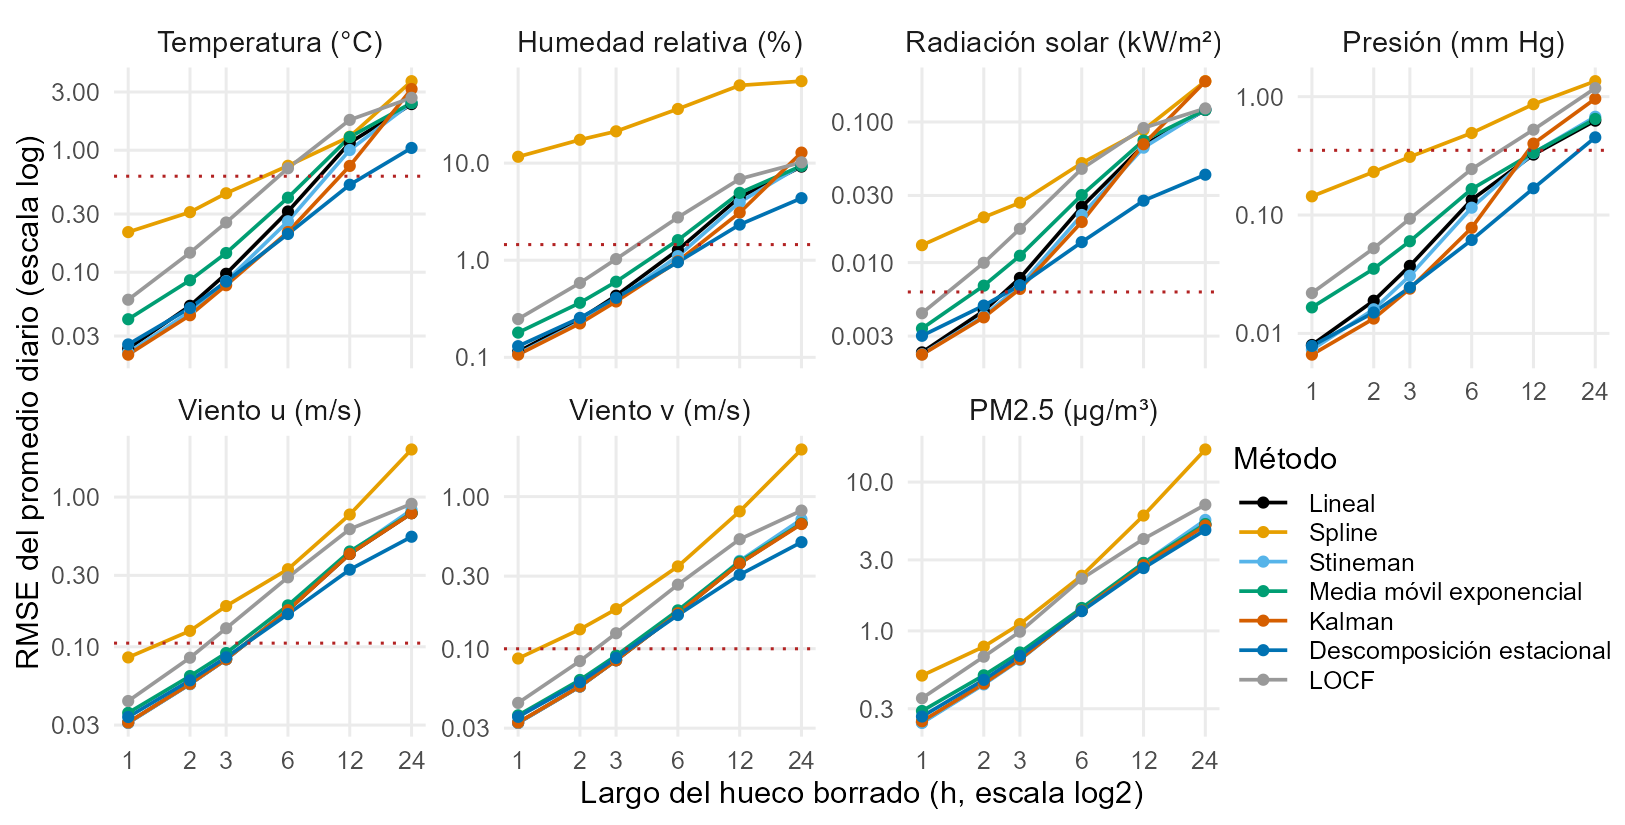
\includegraphics[width=0.95\textwidth]{figuras/rmse_imputacion_informe.png}
\caption{Error (RMSE) del promedio diario según el método de imputación y el largo del hueco borrado, en tramos completos de 2021–2023 (13 estaciones, 5 repeticiones, 2\,730 series por método). Escalas logarítmicas; la línea punteada es el umbral de error tolerado. PM2.5 solo como diagnóstico.}
\label{fig:imputacion}
\end{figure}

La Tabla~\ref{tbl:b-exclusiones} detalla las causas de exclusión que resume la Tabla~\ref{tbl:exclusiones} (Sección~\ref{sec:muestra}).

\begin{table}[H]
\centering\small
\caption{Causas de exclusión por estación, temporada y año (2021–2025): días-estación posibles, sin PM2.5 suficiente (a), con meteorología imputada (c), con 5–8 meteorológicas faltantes (d) y previos a una reubicación (e), y porcentaje de superación en (b) y (c).}
\label{tbl:b-exclusiones}
\begin{tabular}{lrrrrrrr}
\toprule
Grupo & Días posibles & (a) n (\%) & (c) n (\%) & (d) n & (e) n & \% superación (b) & \% superación (c)\\
\midrule
CE & 1\,826 & 268 (14.7) & 100 (5.5) & 3 & 0 & 33.7 & 58.0\\
NE & 1\,826 & 124 (6.8) & 550 (30.1) & 7 & 413 & 29.3 & 27.8\\
NE2 & 1\,826 & 608 (33.3) & 240 (13.1) & 3 & 0 & 33.5 & 21.7\\
NO & 1\,826 & 1\,046 (57.3) & 128 (7.0) & 2 & 147 & 34.8 & 18.8\\
NO2 & 1\,826 & 289 (15.8) & 1\,023 (56.0) & 5 & 0 & 9.8 & 22.7\\
NTE & 1\,826 & 234 (12.8) & 925 (50.7) & 78 & 141 & 18.7 & 16.6\\
NTE2 & 1\,826 & 128 (7.0) & 7 (0.4) & 2 & 0 & 23.3 & 14.3\\
SE & 1\,826 & 285 (15.6) & 148 (8.1) & 22 & 232 & 15.4 & 28.4\\
SE2 & 1\,826 & 140 (7.7) & 206 (11.3) & 6 & 0 & 48.4 & 29.6\\
SE3 & 1\,826 & 249 (13.6) & 337 (18.5) & 3 & 0 & 16.9 & 27.0\\
SO & 1\,826 & 247 (13.5) & 277 (15.2) & 36 & 259 & 46.8 & 33.6\\
SO2 & 1\,826 & 261 (14.3) & 169 (9.3) & 1 & 0 & 20.0 & 9.5\\
SUR & 1\,826 & 467 (25.6) & 82 (4.5) & 21 & 183 & 9.6 & 9.8\\
\midrule
Seca-fría & 7\,813 & 1\,367 (17.5) & 1\,488 (19.0) & 91 & 319 & 38.3 & 34.8\\
Seca-cálida & 5\,980 & 1\,028 (17.2) & 1\,037 (17.3) & 78 & 462 & 36.1 & 29.0\\
Lluvias & 9\,945 & 1\,951 (19.6) & 1\,667 (16.8) & 20 & 594 & 12.8 & 10.0\\
\midrule
2021 & 4\,745 & 596 (12.6) & 1\,186 (25.0) & 99 & 1\,321 & — & —\\
2022 & 4\,745 & 468 (9.9) & 526 (11.1) & 5 & 54 & — & —\\
2023 & 4\,745 & 725 (15.3) & 604 (12.7) & 2 & 0 & — & —\\
2024 & 4\,758 & 1\,118 (23.5) & 843 (17.7) & 1 & 0 & — & —\\
2025 & 4\,745 & 1\,439 (30.3) & 1\,033 (21.8) & 82 & 0 & — & —\\
\bottomrule
\end{tabular}
\end{table}

\begin{table}[H]
\centering\small
\caption{Reglas de limpieza horaria, en el orden en que se aplican, y horas anuladas en las 15 variables (2020–2025). Fuente: \texttt{data/clean/README.md} y \texttt{tabla\_informe\_limpieza.csv}.}
\label{tbl:b-limpieza}
\begin{tabularx}{\textwidth}{>{\raggedright\arraybackslash}p{4.4cm}L>{\raggedleft\arraybackslash}p{2.6cm}}
\toprule
Regla (bandera) & Criterio & Horas anuladas\\
\midrule
Rango duro (F) & Fuera del rango de operación (contaminantes) o del fabricante (meteorología) & 2\,409\\
Notas del PDF de SIMA (P) & Límites anuales que indica SIMA & 116\\
Saturación del sensor (L) & |TOUT| ≥ 49.9\,°C & 25\\
Salto horario (S) & |ΔTOUT| > 10\,°C o |ΔPRS| > 10\,mm\,Hg en una hora & 2\,576\\
PM2.5 > PM10 (R) & Se anulan las dos & 74\\
Racha de valores idénticos (K) & ≥ 24\,h iguales en contaminantes, TOUT, PRS y RH & 13\,598\\
Consistencia espacial, D14 (E) & TOUT a > 10\,°C o RH a > 40\,pp de la mediana de la red (≥ 5 estaciones) & 450 TOUT y 4\,120 RH\\
Radiación de madrugada, D15 (M) & Media de SR entre 00 y 04\,h > 0.02\,kW/m²: se anula todo el día & 49\,491\\
Viento contra la red, D15 (E) & WSR > mediana de la red + 30\,km/h; ≥ 3 horas anulan el día & 4\,426 horas de WSR\\
\bottomrule
\end{tabularx}
\end{table}

Las reglas se aplican en el orden de la Tabla~\ref{tbl:b-limpieza}, sobre los valores horarios observados y antes de imputar. Las horas anuladas por consistencia espacial, saturación o radiación de madrugada nunca se imputan. Todo valor imputado se revalida con las mismas reglas y, si incumple alguna, vuelve a faltante (bandera X); nunca se modifica un valor original válido. La consistencia espacial se repite hasta que ninguna lectura conservada incumple respecto de su propia mediana de la red, y sus umbrales se eligieron con la distribución de las desviaciones y un análisis de sensibilidad (8, 10 y 15\,°C; 30, 40 y 50 puntos porcentuales). El detalle completo, con las cifras por estación, está en \texttt{data/clean/README.md}. La Tabla~\ref{tbl:b-diccionario} resume las variables y sus transformaciones; los diccionarios completos se encuentran en el repositorio.

\begin{table}[H]
\centering\small
\caption{Variables de la base diaria v2 que usa el modelo (\texttt{data/clean/v2/diario\_v2\_imputado\_2021\_2025.csv}).}
\label{tbl:b-diccionario}
\begin{tabularx}{\textwidth}{>{\raggedright\arraybackslash}p{5.4cm}L}
\toprule
Variable & Descripción\\
\midrule
\texttt{estacion}, \texttt{fecha}, \texttt{anio}, \texttt{temporada} & Clave del día-estación y temporada (seca-fría nov–feb, seca-cálida mar–may, cálida-húmeda o lluvias jun–oct)\\
\texttt{PM2.5} & Media diaria con ≥ 18\,h observadas (µg/m\textsuperscript{3}); no se imputa\\
\texttt{supera\_25} & 1 si PM2.5 > 25\ugm{} (referencia fija)\\
\texttt{TOUT}, \texttt{RH}, \texttt{SR}, \texttt{PRS} & Media diaria de temperatura (°C), humedad (\%), radiación (kW/m²) y presión (mm\,Hg)\\
\texttt{viento\_u}, \texttt{viento\_v}, \texttt{viento\_rapidez\_ms} & Componentes y rapidez media diaria del viento (m/s)\\
\texttt{horas\_lluvia} & Horas del día con lluvia (0–24)\\
\texttt{imp\_TOUT}, \texttt{imp\_RH}, … (una por variable) & 1 si la variable de ese día se imputó a nivel diario\\
\texttt{sitio\_valido} & 0 en los días previos a la reubicación de la estación (D23)\\
\bottomrule
\end{tabularx}
\end{table}

% ----------------------- ANEXO C -----------------------
\anexo{Anexo C. Diagnósticos complementarios}
\iniciaanexo{C}
La Tabla~\ref{tbl:puente} detalla el paso de la etapa 3 a la etapa 4 (Sección~\ref{sec:validacion}), y la Tabla~\ref{tbl:robustez}, las variantes de la Sección~\ref{sec:robustez}.

\begin{table}[H]
\centering\small
\caption{Tabla puente de la etapa 3 (datos-v1.2) al análisis final de la etapa 4 (base v2): tamaño de entrenamiento y de prueba, porcentaje de superación en la prueba, AUC de M0 y M1 y \dauc{} con IC 95\,\% (bootstrap por bloques de 14 días, 1\,000 réplicas).}
\label{tbl:puente}
\begin{tabularx}{\textwidth}{cLrrrrr}
\toprule
Paso & Cambio & n entren. / prueba & \% sup. & AUC M0 & AUC M1 & \dauc{} [IC 95\,\%]\\
\midrule
0 & Etapa 3 (datos-v1.2) & 10\,170 / 5\,220 & 27.2 & 0.722 & 0.792 & 0.070 [0.047, 0.094]\\
1 & + respuesta solo con horas observadas (D18) & 9\,983 / 4\,978 & 28.3 & 0.716 & 0.790 & 0.074 [0.051, 0.098]\\
2 & + imputación horaria de la meteorología (D19) & 10\,024 / 4\,987 & 28.4 & 0.717 & 0.790 & 0.074 [0.050, 0.098]\\
3 & + imputación diaria con la mediana de la red ajustada (D20) & 12\,340 / 6\,863 & 26.2 & 0.709 & 0.791 & 0.081 [0.055, 0.109]\\
4 & + entrenamiento sin días previos a la reubicación (D23) = análisis final & 10\,965 / 6\,863 & 26.2 & 0.713 & 0.792 & 0.079 [0.054, 0.104]\\
\bottomrule
\end{tabularx}
\end{table}

\begin{table}[H]
\centering\small
\caption{\dauc{} (M1 − M0) en la prueba 2024–2025 según el análisis, con IC 95\,\% por bootstrap por bloques de 14 días salvo que se indique. Las cuatro últimas filas son sensibilidades posteriores a la evaluación; la última, de la fase F (Sección~\ref{sec:logistica}).}
\label{tbl:robustez}
\begin{tabularx}{\textwidth}{Lrrrrr}
\toprule
Análisis & n entrenamiento & n prueba & AUC M0 & AUC M1 & \dauc{} [IC 95\,\%]\\
\midrule
Análisis final (LDA) & 10\,965 & 6\,863 & 0.713 & 0.792 & 0.079 [0.054, 0.104]\\
Regresión logística & 10\,965 & 6\,863 & 0.721 & 0.792 & 0.071 [0.047, 0.095]\\
Bloques de 7 días & 10\,965 & 6\,863 & 0.713 & 0.792 & 0.079 [0.054, 0.103]\\
Bloques de 28 días (versión conservadora) & 10\,965 & 6\,863 & 0.713 & 0.792 & 0.079 [0.045, 0.110]\\
MICE (m = 20; 4\,000 réplicas) & 10\,965 & 6\,863 & 0.713 & 0.791 & 0.078 [0.055, 0.103]\\
Imputación diaria solo con ≤ 2 faltantes & 10\,408 & 6\,801 & 0.713 & 0.789 & 0.077 [0.052, 0.102]\\
Respuesta con PM2.5 interpolado ≤ 3\,h & 11\,180 & 7\,160 & 0.714 & 0.793 & 0.079 [0.053, 0.105]\\
Sin imputación diaria (casos completos) & 8\,995 & 4\,987 & 0.720 & 0.791 & 0.071 [0.047, 0.096]\\
Radiación imputada truncada en 0 & 10\,965 & 6\,863 & 0.713 & 0.792 & 0.079 [0.054, 0.105]\\
Reubicaciones según SIMA & 11\,365 & 6\,863 & 0.710 & 0.791 & 0.081 [0.054, 0.107]\\
Sin la estación NO2 & 9\,971 & 6\,325 & 0.715 & 0.797 & 0.082 [0.056, 0.108]\\
Logística con splines (GAM) & 10\,965 & 6\,863 & 0.721 & 0.811 & 0.090 [0.060, 0.120]\\
\bottomrule
\end{tabularx}
\end{table}

La Figura~\ref{fig:magnitud} desglosa la clasificación según el PM2.5 observado (Sección~\ref{sec:desempeno}).

\begin{figure}[H]
\centering
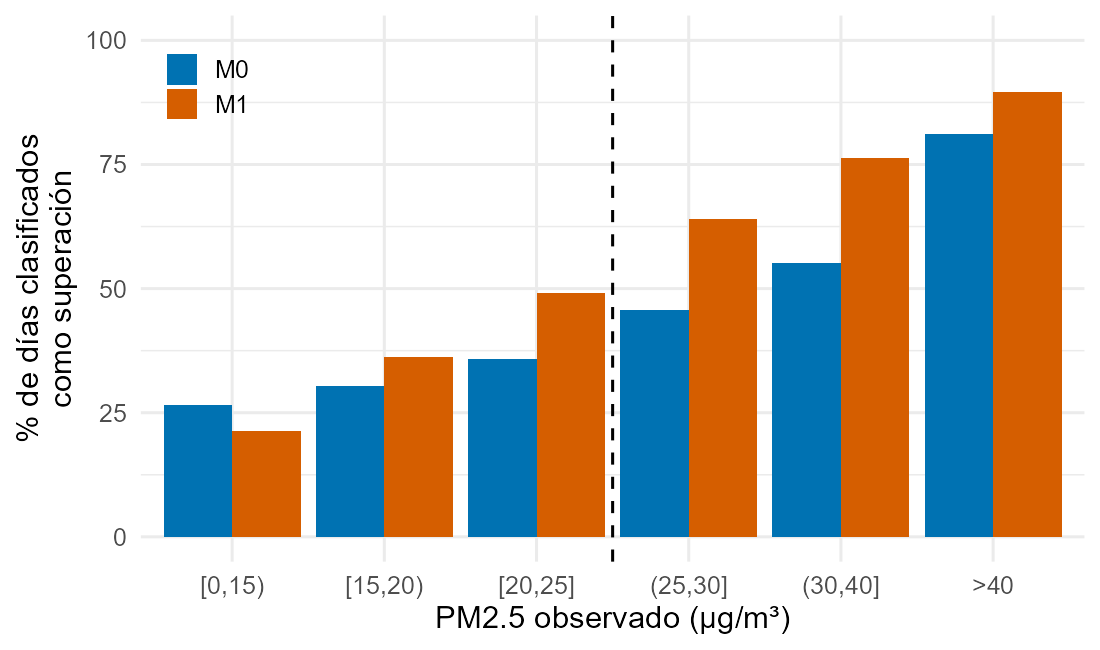
\includegraphics[width=0.58\textwidth]{figuras/errores_magnitud_informe.png}
\caption{Porcentaje de días-estación clasificados como superación según el PM2.5 observado, para M0 y M1 (prueba 2024–2025, n = 6\,863). Por debajo de 25\ugm{} son falsas alarmas y por encima, detecciones.}
\label{fig:magnitud}
\end{figure}

La Figura~\ref{fig:linealidad} respalda la revisión de la linealidad de la Sección~\ref{sec:logistica}: la temperatura, la rapidez del viento y la humedad se apartan de la recta, y la presión y la lluvia casi no. La Figura~\ref{fig:cortes} muestra que, al subir el corte, la sensibilidad baja más rápido de lo que sube el valor predictivo positivo (Sección~\ref{sec:umbral}).

\begin{figure}[H]
\centering
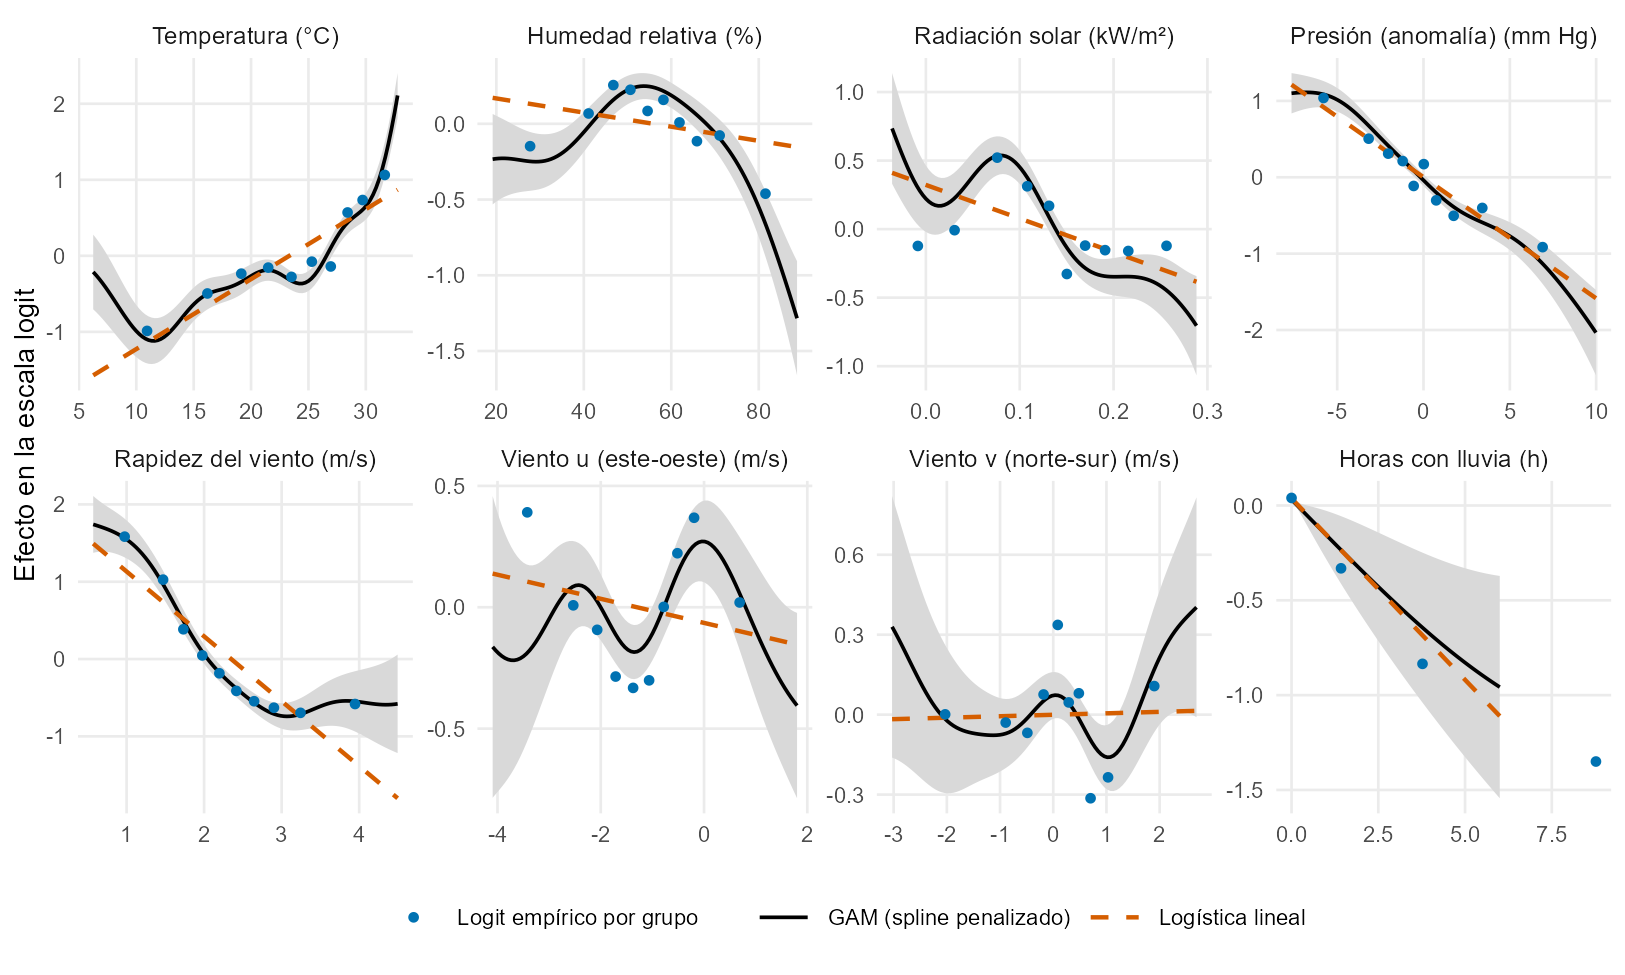
\includegraphics[width=0.95\textwidth]{figuras/linealidad_logit_informe.png}
\caption{Linealidad en la escala logit de las ocho variables meteorológicas en M1 logístico (entrenamiento 2021–2023, n = 10\,965): función del GAM con banda de ± 2 errores estándar (calculada bajo independencia, por lo que es demasiado estrecha), término lineal de la logística y logits empíricos por decil (en la lluvia, días sin lluvia y cuartiles de los días con lluvia), ajustados por estación, temporada y las demás variables. Las curvas están centradas: solo importa su forma.}
\label{fig:linealidad}
\end{figure}

\begin{figure}[H]
\centering
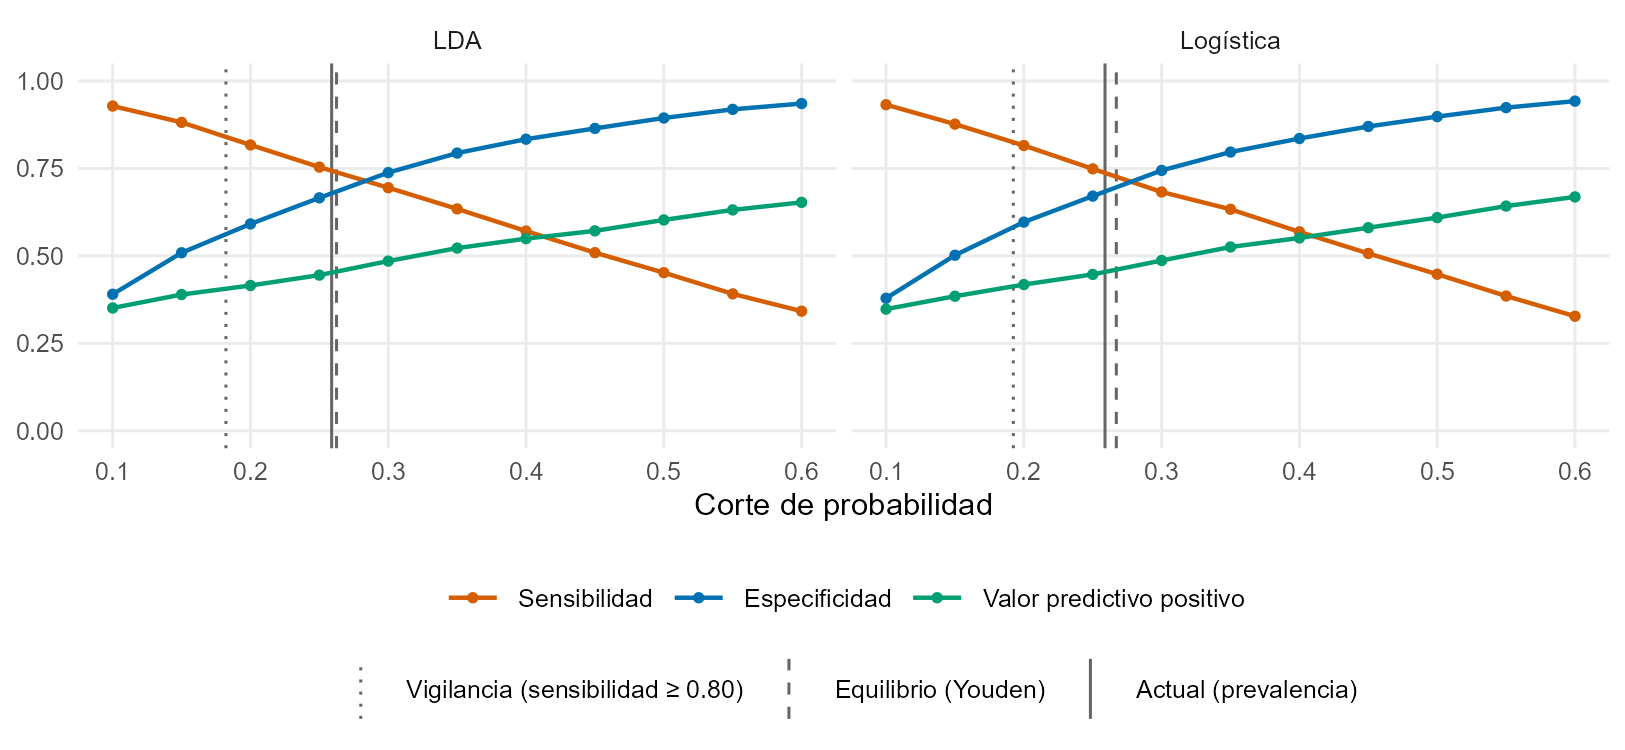
\includegraphics[width=0.95\textwidth]{figuras/metricas_por_corte_informe.png}
\caption{Sensibilidad, especificidad y valor predictivo positivo de M1 en la prueba 2024–2025 (n = 6\,863) según el corte de probabilidad, con los tres cortes elegidos sin usar la prueba (Sección~\ref{sec:umbral}).}
\label{fig:cortes}
\end{figure}

\begin{table}[H]
\centering\small
\caption{Errores de M1 por estación en la prueba 2024–2025 (corte 0.259): días, porcentaje de superación, sensibilidad, especificidad y razón entre el error cuadrático observado y el esperado. † NO2 incluye 272 días del periodo con PM2.5 anómalo (enero de 2024–enero de 2025), sin ninguna superación.}
\label{tbl:c-errores}
\begin{tabular}{lrrrrr}
\toprule
Estación & Días & \% superación & Sensibilidad & Especificidad & Error observado / esperado\\
\midrule
NO & 51 & 49.0 & 0.84 & 0.54 & 1.00\\
SE2 & 705 & 42.8 & 0.95 & 0.25 & 0.90\\
SO & 521 & 39.3 & 0.91 & 0.38 & 1.00\\
NE2 & 218 & 37.2 & 0.85 & 0.51 & 1.05\\
CE & 592 & 30.9 & 0.83 & 0.53 & 1.05\\
NE & 657 & 30.7 & 0.78 & 0.74 & 0.99\\
NTE2 & 670 & 27.3 & 0.69 & 0.82 & 1.13\\
SO2 & 566 & 26.5 & 0.41 & 0.76 & 1.49\\
SE3 & 577 & 25.1 & 0.73 & 0.66 & 1.17\\
NTE & 662 & 16.6 & 0.54 & 0.83 & 1.11\\
SE & 569 & 16.5 & 0.61 & 0.83 & 1.08\\
NO2† & 538 & 11.2 & 0.52 & 0.66 & 0.94\\
SUR & 537 & 11.0 & 0.34 & 0.88 & 1.04\\
\bottomrule
\end{tabular}
\end{table}

La Tabla~\ref{tbl:c-errores} muestra que, con un solo corte para toda la red, el modelo detecta casi todas las superaciones donde son frecuentes (SE2, SO) a costa de muchas falsas alarmas, y pierde muchas donde son raras (SUR) y en SO2. En NO2, la superación baja no es solo una característica del sitio: la mitad de sus días de prueba cae en el periodo con PM2.5 anómalo, sin ninguna superación (22.6\,\% en el resto). Es la razón de recomendar cortes por estación, una vez resuelto el caso de NO2. El error supera al esperado sobre todo en SO2 (1.49) y SE3 (1.17).

\begin{table}[H]
\centering\small
\caption{Calibración de M1 en la prueba 2024–2025: probabilidad media y frecuencia observada de superación por decil de probabilidad.}
\label{tbl:c-calibracion}
\begin{tabular}{lrrrrrrrrrr}
\toprule
Decil & 1 & 2 & 3 & 4 & 5 & 6 & 7 & 8 & 9 & 10\\
\midrule
Probabilidad media & 0.02 & 0.05 & 0.08 & 0.12 & 0.18 & 0.25 & 0.32 & 0.43 & 0.58 & 0.79\\
Frecuencia observada & 0.02 & 0.06 & 0.09 & 0.13 & 0.22 & 0.23 & 0.29 & 0.39 & 0.50 & 0.70\\
\bottomrule
\end{tabular}
\end{table}

\begin{table}[H]
\centering\small
\caption{Recalibración de M1 por temporada en la prueba (regresión logística de la superación sobre el logit de la probabilidad; ideal: intercepto 0 y pendiente 1).}
\label{tbl:c-cal-temporada}
\begin{tabular}{lrrrrr}
\toprule
Temporada & Días & Probabilidad media & Frecuencia observada & Intercepto & Pendiente\\
\midrule
Seca-fría (nov–feb) & 2\,372 & 0.41 & 0.36 & −0.34 & 0.76\\
Seca-cálida (mar–may) & 1\,693 & 0.36 & 0.40 & 0.08 & 0.75\\
Lluvias (jun–oct) & 2\,798 & 0.12 & 0.10 & −0.81 & 0.69\\
\bottomrule
\end{tabular}
\end{table}

La Tabla~\ref{tbl:c-calibracion} y la Tabla~\ref{tbl:c-cal-temporada} muestran que las probabilidades de M1 ordenan bien los días (la frecuencia observada crece con el decil), pero son demasiado extremas: la pendiente de la recalibración es menor que 1 en las tres temporadas.

\begin{table}[H]
\centering\small
\caption{Días-estación por año en el modelado: muestra de la etapa 3 (datos-v1.2) frente al análisis final de la etapa 4 (base v2).}
\label{tbl:c-dias}
\begin{tabular}{lrrr}
\toprule
Año & Etapa 3 & Etapa 4 & Diferencia\\
\midrule
2021 & 2\,863 & 2\,729 & −134\\
2022 & 3\,802 & 4\,218 & 416\\
2023 & 3\,505 & 4\,018 & 513\\
2024 & 2\,894 & 3\,639 & 745\\
2025 & 2\,326 & 3\,224 & 898\\
\bottomrule
\end{tabular}
\end{table}

La Tabla~\ref{tbl:c-dias} muestra que la base final gana días en todos los años salvo 2021, donde los días previos a las reubicaciones salen del entrenamiento (D23). La Figura~\ref{fig:c-no2} respalda la pregunta para SIMA sobre el equipo de PM2.5 de NO2, y la Figura~\ref{fig:c-coef} completa la Figura~\ref{fig:coef} con las indicadoras de estación: SO es la única con un efecto estable mayor que el de CE (la referencia), y el de SE2 no se distingue del de CE.

\begin{figure}[H]
\centering
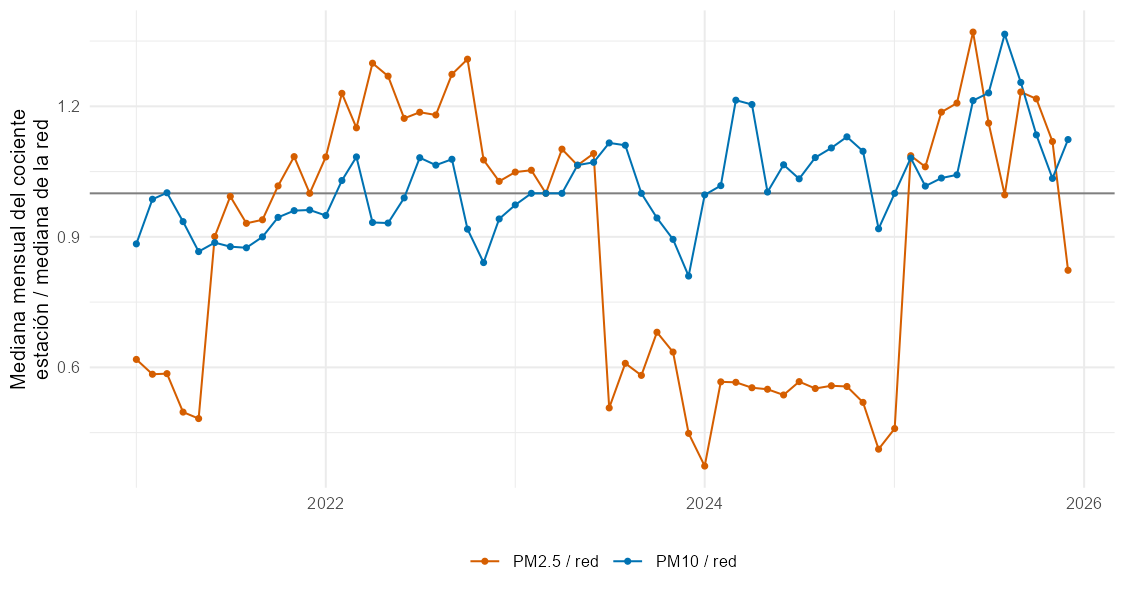
\includegraphics[width=0.75\textwidth]{figuras/no2_relativo_informe.png}
\caption{PM2.5 y PM10 de NO2 (García) divididos entre la mediana de la red, por mes, 2021–2025. El PM2.5 baja a la mitad mientras el PM10 sigue en su nivel, lo que apunta a un problema del equipo de PM2.5.}
\label{fig:c-no2}
\end{figure}

\begin{figure}[H]
\centering
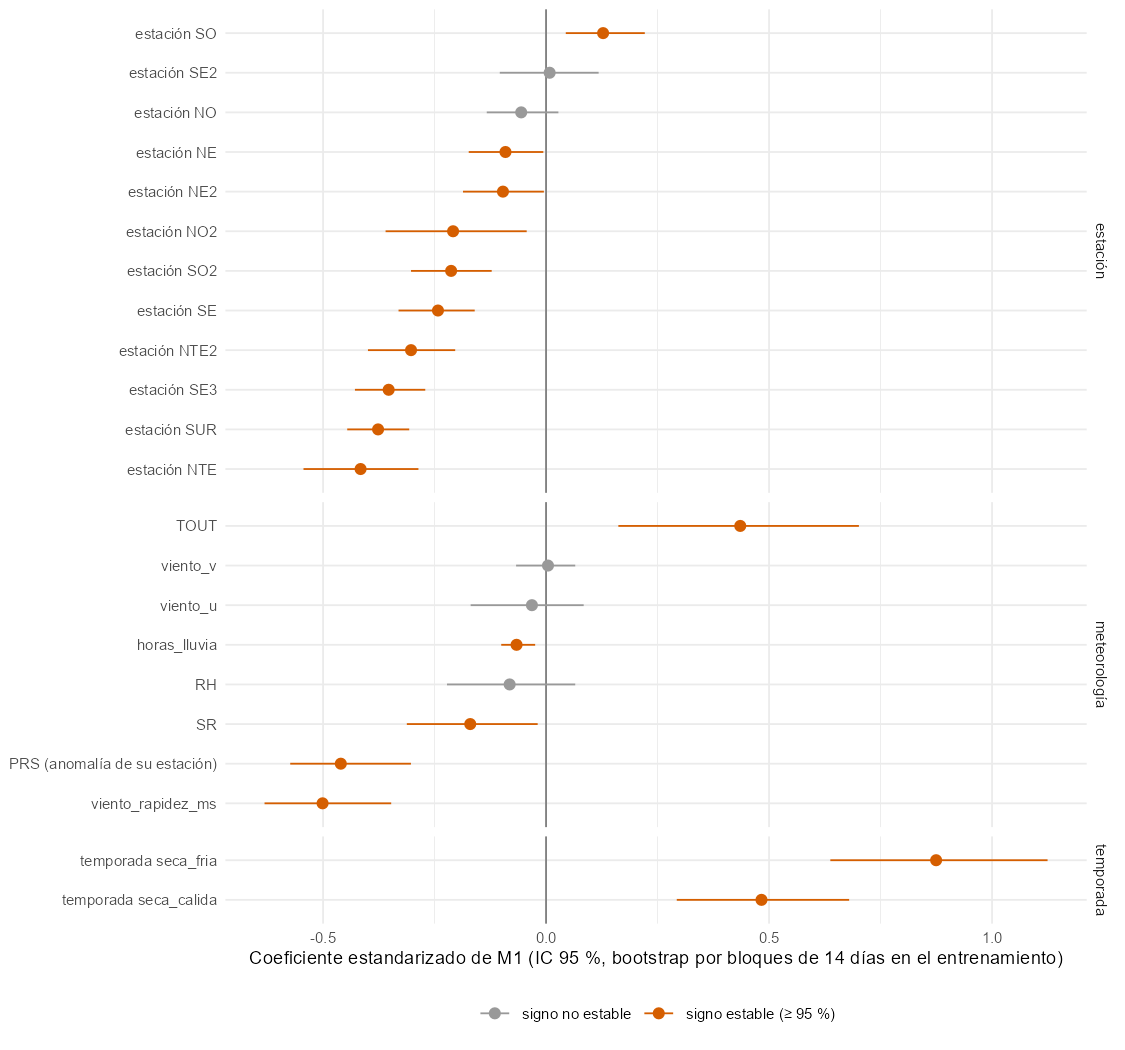
\includegraphics[width=0.78\textwidth]{figuras/coeficientes_ic_informe.png}
\caption{Coeficientes estandarizados de M1 con todas las indicadoras de estación, e IC 95\,\% por bootstrap por bloques de 14 días en el entrenamiento (1\,000 réplicas).}
\label{fig:c-coef}
\end{figure}

% ----------------------- ANEXO D -----------------------
\anexo{Anexo D. Declaratoria de uso de IA (Opción B)}
\begin{itemize}
\item \textbf{Herramientas:} Claude (Anthropic): Claude Opus y Claude Code; ChatGPT y Codex (OpenAI).
\item \textbf{Uso realizado:}
  \begin{itemize}
  \item Claude Opus: planeación de cada etapa, búsqueda y verificación de literatura, decisiones de análisis propuestas, revisión de resultados, redacción de los informes, verificación de los hallazgos de la auditoría final y conversión de este informe a LaTeX.
  \item Claude Code: scripts de R de limpieza, imputación, modelos, validaciones y figuras (\texttt{scripts/02} a \texttt{10}), aplicación Shiny, armado del documento en Quarto y verificación de cifras y citas.
  \item Codex: revisiones independientes de código y cifras de las etapas anteriores, apoyo en la redacción y el formato, preparación de la entrega de la etapa 3 en LaTeX y edición de esta declaratoria a partir de las aportaciones confirmadas por el equipo.
  \item Uso por integrantes: Leonardo Orozco coordinó el trabajo con Claude Opus, Claude Code y Codex para discutir el análisis, desarrollar y revisar el código, contrastar observaciones y preparar los informes. Ignacio Kume utilizó herramientas de IA con razonamiento en profundidad para desarrollar preguntas que el equipo empleó para complementar la exposición y distintas partes del reto. Pablo Alonso Robles Nava utilizó Claude como apoyo analítico para realizar auditorías recurrentes del trabajo y preparar la presentación final. En etapas anteriores, integrantes del equipo también utilizaron Claude y ChatGPT para los borradores de contexto y las fichas de lectura a partir de los PDF de las fuentes.
  \end{itemize}
\item \textbf{Secciones:} todo el informe y el código del repositorio.
\item \textbf{Validación realizada por los estudiantes:} a lo largo del proyecto, Leonardo Orozco contrastó cifras con los CSV, ejecutó el cuaderno de auditoría, revisó las decisiones de modelado y probó la interfaz. Ignacio Kume y Daniel Ayala leyeron los artículos correspondientes a sus fichas; Ignacio verificó fuentes del contexto ambiental y probó la interfaz, y Daniel revisó que el banco de preguntas fuera coherente con los resultados. Pablo Alonso Robles Nava revisó la redacción, investigó el fundamento de los métodos estadísticos y participó en la interpretación de los resultados. Las preguntas desarrolladas por Ignacio y las auditorías coordinadas por Pablo apoyaron la revisión del trabajo y la preparación de la exposición. Estas aportaciones no implican que cada integrante haya reproducido por separado todos los cálculos del informe final.
\item El equipo asume la responsabilidad sobre el contenido entregado, sus decisiones metodológicas, sus citas y sus limitaciones. La asistencia de IA no sustituye la revisión del equipo ni constituye por sí misma una validación de los resultados.
\end{itemize}


\end{document}
